%\documentclass[11pt,a4paper]{article}
\documentclass[11pt
  , a4paper
  , article
  , oneside
%  , twoside
%  , draft
]{memoir}

\usepackage{control}
\usepackage[numbers]{natbib}


\begin{document}

\newcommand{\technumber}{
  RAON Control-Document Series\\
  Revision : v1.0,   Release : Jan. 02. 2015}
\title{\textbf{SNMP 메뉴얼}}

\author{박미정\thanks{mijoy0909@ibs.re.kr} \\

  Rare Isotope Science Project\\
  Institute for Basic Science, Daejeon, South Korea
}
\date{\today}

\renewcommand{\maketitlehooka}{\begin{flushright}\textsf{\technumber}\end{flushright}}
%\renewcommand{\maketitlehookb}{\centering\textsf{\subtitle}}
%\renewcommand{\maketitlehookc}{C}
%\renewcommand{\maketitlehookd}{D}

\maketitle

\begin{abstract}
SNMP는 IP 네트워크에서 장치를 관리하기 위한 공식 인터넷 표준 프로토콜(Official Internet Standards Protocol)\citep{oisp}이다. 본 문서는 SNMP설정 및 SNMP를 이용한 모니터링 및 다양한 네트워크 환경에서 SNMP의 버전별 응답시간에 관해 설명한다. 
\end{abstract}

\chapter{SNMP란?}
SNMP(Simple Network Management Protocol)는 IP네트워크 상의 장비들을 관리하고 모니터링하기 위한 인터넷 표준 프로토콜이다. SNMP는 Manager와 Agent로 구성되어있으며, Manager는 Agent에게 장비의 필요한 정보를 요청하거나, 장비의 정보를 변경한다. Manager는 NMS(Network Management Stations)로 표현되기도 한다. Agent는 Manager가 요청한 정보를 제공하고, 시스템 충돌이나 재부팅 등의 장비에 영향을 미치거나 발생한 Event를 비동기적으로 알리기 위해 Trap 메시지를 보낸다. 이들의 관계는 그림 \ref{fig:relationship_m_a}\citep{essential_snmp}과 같다. 이는 원래 NMS와 Agent의 관계이지만 본 연구에서는 Manager와 Agent의 관계로 재구성하였다.
\begin{figure}[h!]
  \centering
  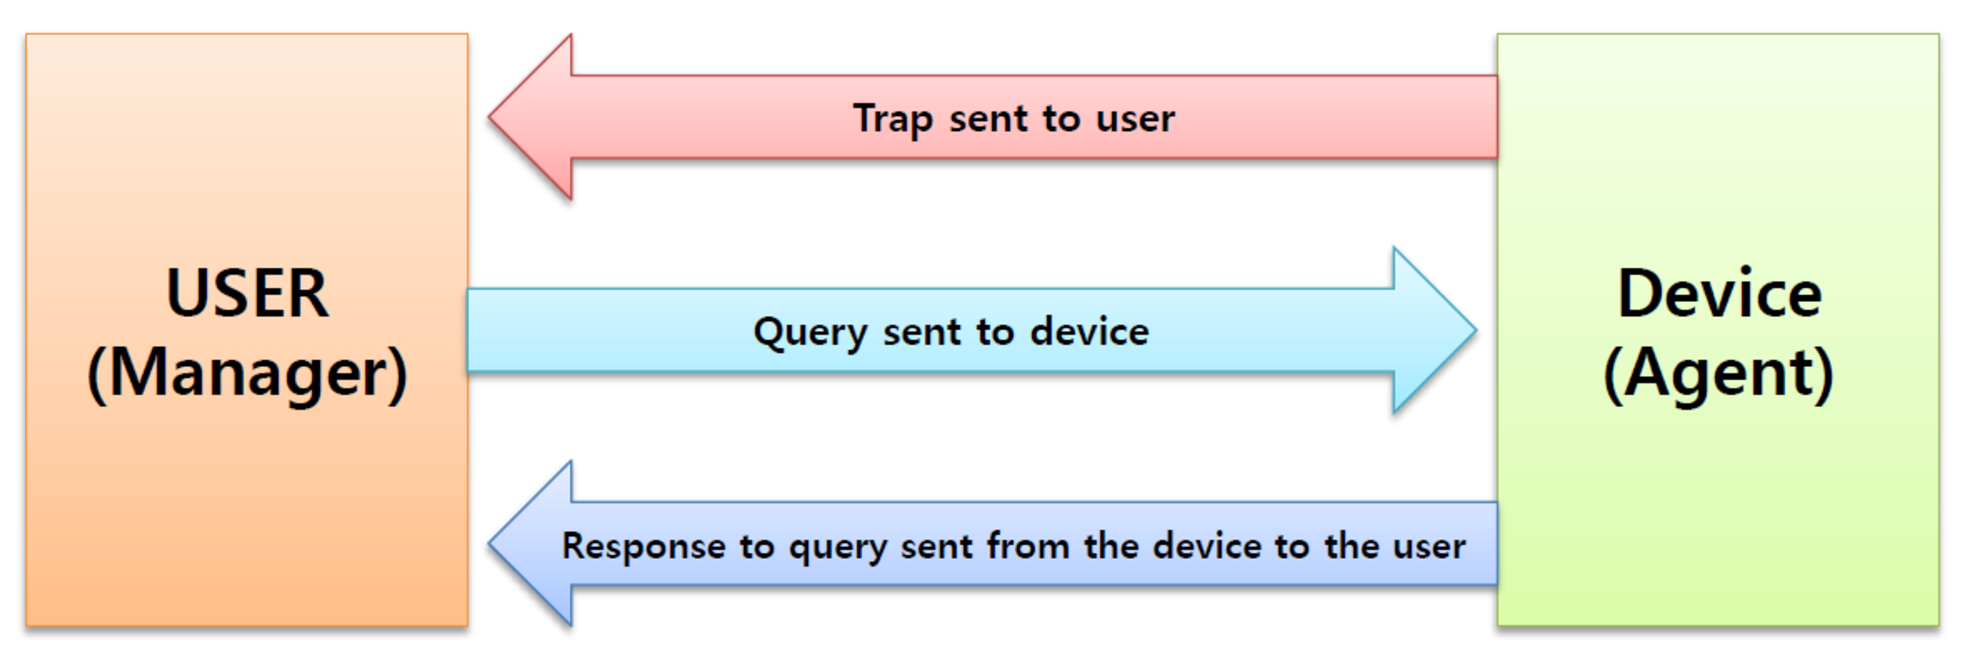
\includegraphics[width=0.65\textwidth]{./images/relationship_m_a.eps}
  \caption{Manager와 Agent의 관계}
  \label{fig:relationship_m_a}   
\end{figure}

\hfil\break
\hfil\break
\hfil\break
\hfil\break

SNMP는 v1/2c/3의 세가지 버전이 있으며, 각 버전들은 인증과 암호화에 따른 차이점이 있다. SNMPv1/2c는 community string을 통해 사용자 인증을 하며, v3는 noAuthNoPriv, authNoPriv, authPriv의 세 종류의 보안 레벨에 따라 username, 암호화 알고리즘인 MD5, SHA로 사용자 인증을 하며, DES, AES 알고리즘을 통해 사용자가 지정한 패스워드 또한 암호화한다. 따라서 인증 및 암호화가 강화되는 v3의 경우 응답시간이 v1/2c에 비해 크다. 버전별 차이점은 표 \ref{table:conparision}\citep{comparison}에서 알 수 있다.

\begin{table}[h!]
\begin{center}
\begin{tabular}{c|c|c|c}\hline
Version & Level & Authentication & Encryption \\ \hline
v1 & noAuthNoPriv & Community string & No \\ \hline
v2c & noAuthNoPriv & Community string & No \\ \hline
 & noAuthNoPriv & Username & No \\ \cline{2-4}
v3 & authNoPriv & MD5 or SHA & No \\ \cline{2-4}
 & authPriv & MD5 or SHA & DES or AES \\ \hline
\end{tabular}
\caption{SNMP 버전별 암호화에 관한 차이점 비교}
  \label{table:conparision}  
\end{center}
\end{table} 

\section{MIB 파일}
SNMP를 사용하기 위해서는 MIB(Management Information Base)파일이 필요하며, 일반적인 TCP/IP관리정보는 MIB-2(RFC 1213)에 포함되어 있고, 특정 장비 관련 정보는 장비제조업체에서 제공한다. 이 MIB파일은 장비에 대한 정보 값 OID(Object Identifiers)를 계층구조로 모아놓은 것으로 앞서 언급된 Manager가 요청하는 정보에 대해 Agent가 제공하는 정보이기도 하다. 

\begin{figure}[h!]
  \centering
  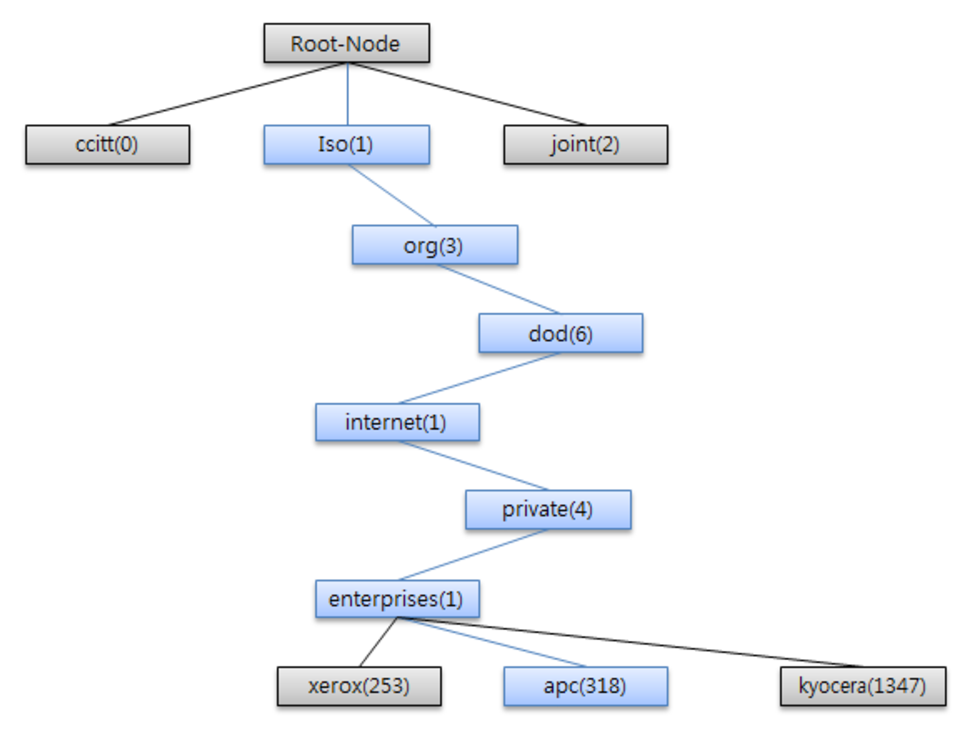
\includegraphics[width=0.65\textwidth]{./images/oid_tree.eps}
  \caption{OID tree}
  \label{fig:oid_tree} 
\end{figure}


그림 \ref{fig:oid_tree}의 OID tree는 ROOT-Node에서 시작하고 밑으로 branch node와 leaf node로 이루어져있다. 예를 들어 apc사의 OID는 1.3.6.1.4.1.318(iso.org.dod.internet\\.private.enterprises.apc)이다. 이러한 트리구조의 MIB는 파일 안에서 그림 \ref{fig:ex_mib}과 같은 포맷을 가진다. MIB파일의 access정도(read-only, read-write, etc...)에 따라 장비에 값을 읽고, 쓸 수 있다.

\begin{figure}[h!]
  \centering
  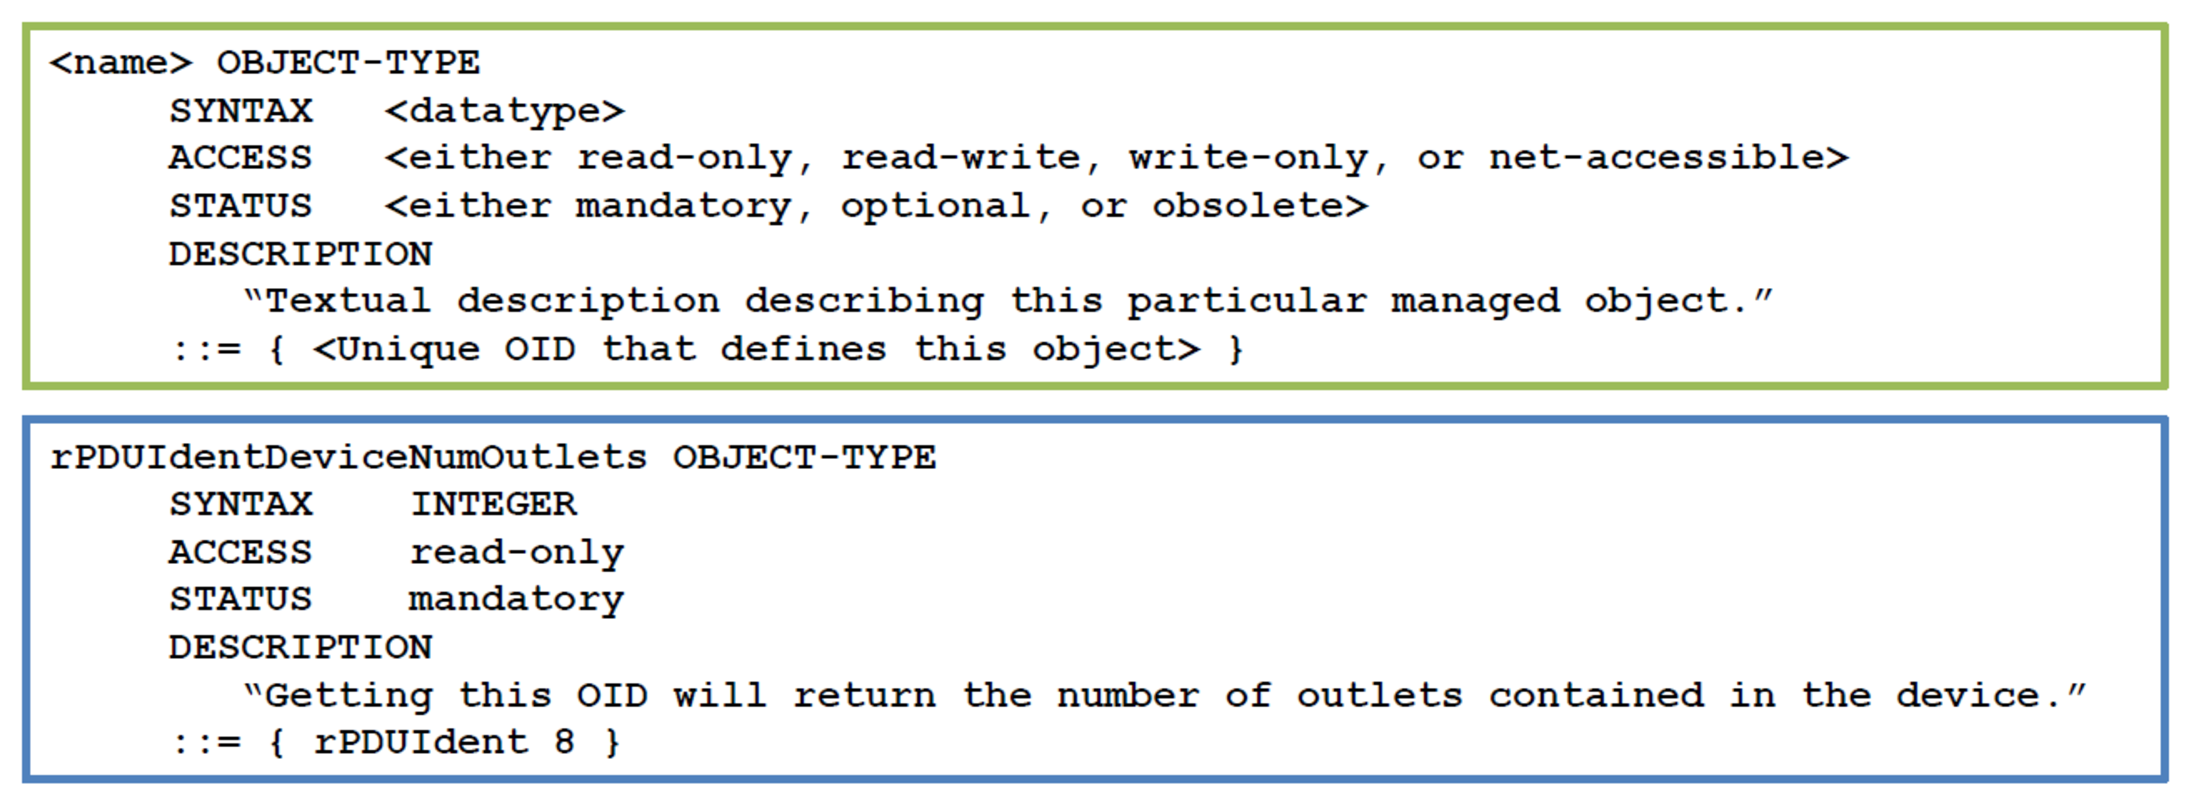
\includegraphics[width=0.8\textwidth]{./images/ex_mib.eps}
  \caption{MIB파일 포맷의 예}
  \label{fig:ex_mib}   
\end{figure}

\chapter{SNMP 사용 방법}
\section{설치}
SNMP를 사용하기 위해서는 아래의 패키지가 설치되어야 한다. 본 문서에서는 NET-SNMP\citep{net_snmp} v5.4.3을 사용하고 있다.
\begin{itemize}
\item NET-SNMP\footnote{* NET-SNMP는 http://www.net-snmp.org/download.html에서 다운받을 수 있다.}
\item snmp snmpd
\item snmp-mibs-downloader
\item libsnmp-dev libsnmp-base libsnmp-perl libsnmp15 
\end{itemize}


\section{SNMP 명령어}

SNMP를 사용하기 위해서는 SNMP명령어\citep{snmp_command}가 필요하고, 명령어는 다음과 같다.
\begin{itemize}
\item get : manager가 agent에게 특정 정보를 요청할 때 사용
\item getnext : get과 동일, 특정 정보의 다음 번 정보를 요청할 때 사용
\item walk : manager가 agnet의 모든 정보를 요청할 때 사용
\item set : manager가 agent의 값을 설정할 때 사용
\item trap : agent에서 비동기적 사건을 manager에게 알리기 위해 사용
\item etc\footnote{* http://www.net-snmp.org/wiki/index.php/Tutorials를 참조 바람}...
\end{itemize}

\section{SNMP 사용}
SNMP명령어를 사용하여 장비의 정보를 읽어오는 방법은 버전에 따라 달라진다.

\begin{itemize}
\item SNMP v1/2c 일 때
\end{itemize}

\begin{lstlisting}[style=termstyle]
snmp(walk, get, trap...) -v (v1/2c) -c (Community String) (HostAddress) (OID) 
\end{lstlisting}

보통 v1/2c의 community string은 제조사에서 public/privacy로 지정해두는데 public은 read-only, privacy는 read-write가 가능하다. 따라서 public에서는 snmpset을 사용할 수 없으며, community string은 사용자가 임의로 설정할 수 있다. v1/2c는 community string을 사용한 사용자 인증 외에는 특별한 보안이 없어 보안에 취약하다는 것을 알 수 있다. 아래는 SNMPv1을 이용해 읽은 localhost의 정보이다.
\begin{lstlisting}[style=termstyle]
mijoy0909@mjpark:~$ snmpwalk -v 1 -c public localhost
RFC1213-MIB::sysDescr.0 = STRING: "Linux mjpark 3.2.0-4-amd64 #1 SMP Debian 3.2.63-2+deb7u2 x86_64"
RFC1213-MIB::sysObjectID.0 = OID: SNMPv2-SMI::enterprises.8072.3.2.10
RFC1213-MIB::sysUpTime.0 = Timeticks: (49138) 0:08:11.38
RFC1213-MIB::sysContact.0 = STRING: "Me <me@example.org>"
RFC1213-MIB::sysName.0 = STRING: "mjpark"
.
.
.
\end{lstlisting}

\begin{itemize}
\item SNMP v3 일 때
\end{itemize}

\begin{lstlisting}[style=termstyle]
snmp(walk, get, trap...) -v 3 -u (Username) -l {Security Level(noAuthNoPriv/authNoPriv/authPrive)} -a {Authentication Protocol(MD5/SHA)} -A (PASSWORD) -x {Privacy Protocol(DES/AES)} -X (PASSWORD) (HostAddress) (OID) 
\end{lstlisting}

다음과 같이 v3의 명령어가 v1/2c에 비해 긴 것을 알 수 있다. 이는 v3에서는 v1/2c와 달리 사용자인증 및 암호를 요구하고 이를 암호화 하기 때문이다. 
SNMPv3를 사용하기 위해서는 Username 및 암호화에 대한 정보를 설정하여야 한다. 장비에 대한 정보 설정은 장비제조업체에서 제공하는 프로그램이나 사이트를 이용하거나 시리얼 통신을 통해 설정 할 수 있다. localhost는 net-snmp의 snmpd를 이용 할 수 있으며, net-snmp의 snmpd를 이용한 localhost의 v3 설정 방법은 다음과 같다. 이 때, 패스워드는 적어도 8자 이상이여야 한다.

\begin{lstlisting}[style=termstyle]
mijoy0909@mjpark:~$ su                                     
root@mjpark:~# service snmpd stop
Stopping network management services: snmpd snmptrapd.
root@mjpark:~# net-snmp-config --create-snmpv3-user
Enter a SNMPv3 user name to create: 
mijoy
Enter authentication pass-phrase: 
[password]
Enter encryption pass-phrase: 
  [press return to reuse the authentication pass-phrase]
[password]
adding the following line to /var/lib/snmp/snmpd.conf:
   createUser test MD5 "[password]" DES [password]
adding the following line to /usr/share/snmp/snmpd.conf:
   rwuser mijoy
root@mjpark:~# service snmpd start
Starting network management services: snmpd.
\end{lstlisting}

위와 같이 net-snmp snmpd를 설정한 후 /usr/share/snmp/snmpd.conf에서 확인하면 아래와 같이 Username이 등록된 것을 알 수 있으며 또한 localhost가 SNMPv3로 읽어지는 것을 확인할 수 있다.\footnote{* http://www.net-snmp.org/docs/README.snmpv3.html 참조 바람}

\begin{lstlisting}[style=termstyle]
rwuser mijoy
\end{lstlisting}

\begin{lstlisting}[style=termstyle]
mijoy0909@mjpark:~$ snmpwalk -v 3 -u mijoy -l authPriv -a MD5 -A  [PASSWORD]  -x DES -X  [PASSWORD]  localhost
RFC1213-MIB::sysDescr.0 = STRING: "Linux mjpark 3.2.0-4-amd64 #1 SMP Debian 3.2.63-2+deb7u2 x86_64"
RFC1213-MIB::sysObjectID.0 = OID: SNMPv2-SMI::enterprises.8072.3.2.10
RFC1213-MIB::sysUpTime.0 = Timeticks: (32928) 0:05:29.28
RFC1213-MIB::sysContact.0 = STRING: "Me <me@example.org>"
RFC1213-MIB::sysName.0 = STRING: "mjpark"
.
.
.
\end{lstlisting}

지금까지 snmpwalk를 이용하여 장비의 모든 정보를 읽어보았고, SNMPv1과 v3의 결과 값이 동일하다는 것을 알 수 있다. snmpwalk와 달리 snmpget을 이용하면 아래와 같이 원하는 정보 값만 읽을 수 있다.
\begin{lstlisting}[style=termstyle]
mijoy0909@mjpark:~$ snmpget -v 1 -c public 10.1.4.182 1.3.6.1.2.1.43.16.5.1.2.1.1
Printer-MIB::prtConsoleDisplayBufferText.1.1 = STRING: "Scan-User Action"
\end{lstlisting}

다음은 snmpset을 이용하여 장비에 원하는 값을 쓰는 방법이다. set역시 walk/get과 마찬가지로 버전에 따른 명령어의 차이가 있다.

\begin{itemize}
\item SNMP v1/2c 일 때
\end{itemize}

\begin{lstlisting}[style=termstyle]
mijoy0909@mjpark:~$ snmpset -v (v1/2c) -c (Community String) (HostAddress) (OID) (datatypes) (value)
\end{lstlisting}

\begin{itemize}
\item SNMP v3 일 때
\end{itemize}

\begin{lstlisting}[style=termstyle]
mijoy0909@mjpark:~$ snmpset -v 3 -u (Username) -l {Security Level(noAuthNoPriv/authNoPriv/authPrive)} -a {Authentication Protocol(MD5/SHA)} -A (PASSWORD) -x {Privacy Protocol(DES/AES)} -X (PASSWORD) (HostAddress) (OID) (datatypes) (value)
\end{lstlisting}

여기서 datatypes는 장비의 정보가 가진 datatypes을 의미하며 snmpset에서 datatypes 옵션은 아래와 같이 정의된다.

\begin{lstlisting}[style=termstyle]
 i: INTEGER 
 u: unsigned INTEGER 
 t: TIMETICKS
 a: IPADDRESS
 o: OBJID
 s: STRING
 x: HEX STRING
 d: DECIMAL STRING
 U: unsigned int64
 I: signed int64
 F: float
 D: double
\end{lstlisting}

APC사의 Power Distribution Unit을 이용한 SNMPv3set 명령어에 대한 예는 아래와 같다. 이 때, 여러 값을 쓸 수 있다.

\begin{lstlisting}[style=termstyle]
snmpset -v 3 -u mijoy -l authPriv -a MD5 -A [PASSWORD] -x DES -X [PASSWORD] 10.1.5.142 sPDUOutletCtl.8 i 2
PowerNet-MIB::sPDUOutletCtl.8 = INTEGER: outletOff(2)
.
.
snmpset -v 3 -u mijoy -l authPriv -a MD5 -A [PASSWORD] -x DES -X [PASSWORD] 10.1.5.142 sPDUOutletCtl.7 i 1 sPDUOutletCtl.8 i 1
PowerNet-MIB::sPDUOutletCtl.7 = INTEGER: outletOn(1)
PowerNet-MIB::sPDUOutletCtl.8 = INTEGER: outletOn(1)
\end{lstlisting}

여기서 지금까지와 달리 OID번호를 이용하지 았다는 것을 알 수 있다. SNMP에서는 OID번호 대신 MIB파일 내의 Object의 이름을 사용하여 장비의 정보를 읽고, 쓸 수 있다. 이 때, 사용하고자하는 장비의 MIB파일과 .snmp/snmp.conf파일(그림 \ref{fig:snmp_conf})을 수정하여야한다.
예를 들어 그림 \ref{fig:pdu_mib}는 APC사 PDU의 MIB파일의 일부분이다. MIB파일의 DEFINITIONS ::= BEGIN에서 MIB파일의 이름을 정의해주고, MIB파일도 똑같은 이름으로 저장해야한다. 따라서 이 MIB파일의 이름은 PowerNet-MIB이다. 

\begin{figure}[h]
  \centering
  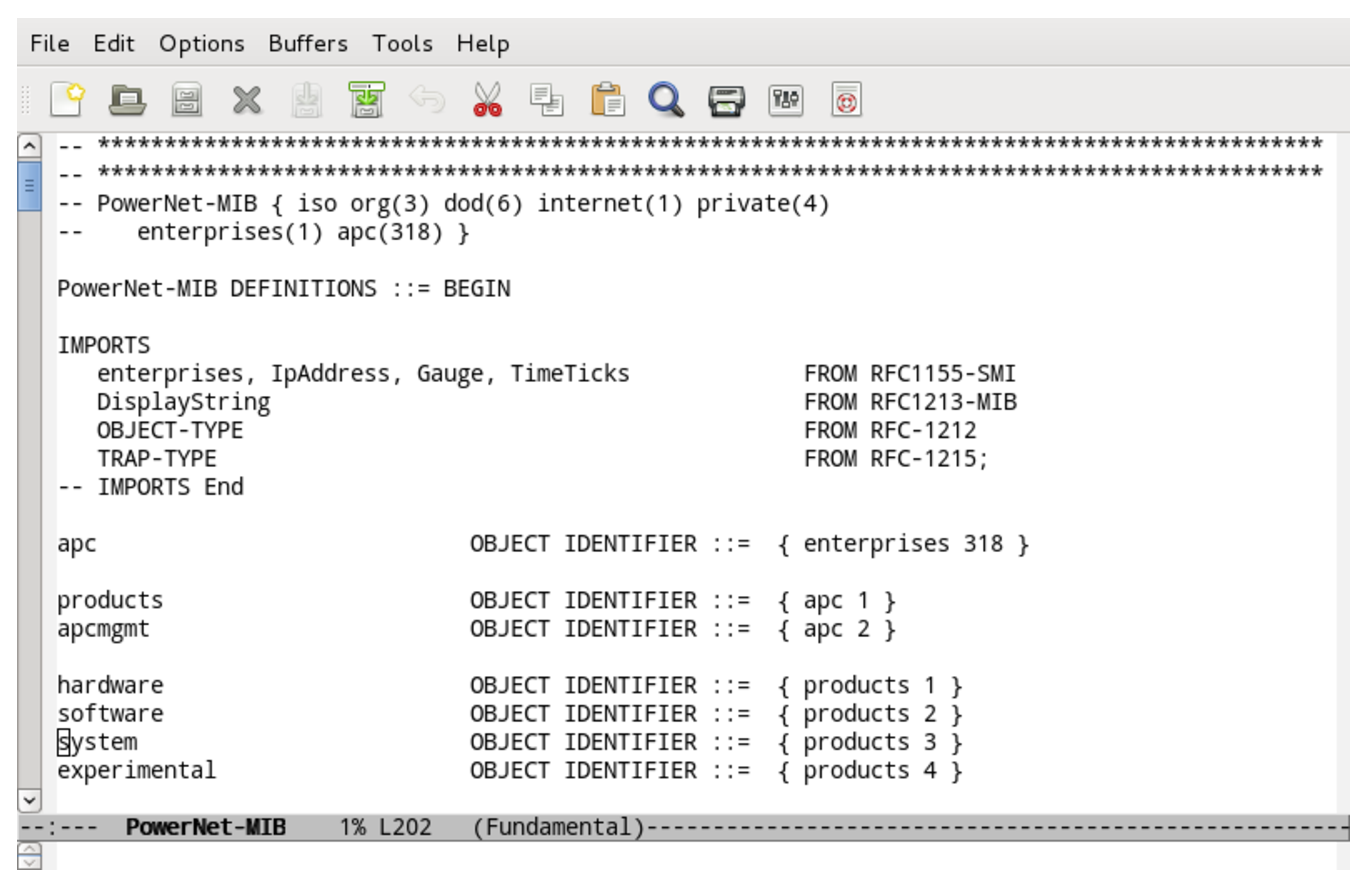
\includegraphics[width=0.99\textwidth]{./images/pdu_mib.eps}
  \caption{APC사 PDU의 MIB파일}
  \label{fig:pdu_mib}   
\end{figure}


\clearpage

snmp.conf파일에는 MIB파일을 등록해주어야한다. 이 과정을 거치면 OID번호가 아닌 Object의 이름으로 장비의 정보를 읽고 쓸 수 있다. 

SNMPv1/2c와 달리 v3의 명령어가 긴 문제를 해결하기 위해서 그림 \ref{fig:snmp_conf}와 같이 snmp.conf파일에 미리 v3에 대한 보안레벨과 암호화 프로토콜을 설정하고 패스워드정보를 저장해둔다면 아래와 같이 간단하게 SNMPv3를 사용할 수 있다.\footnote{* 여러가지 장비의 정보를 설정한 후 사용해봤지만 첫 번째로 저장된 정보에만 간단하게 SNMPv3 사용이 가능하였다. 이는 추가적인 확인이 필요하다. 만약 첫 번째로 저장된 정보에만 가능하다면 v3를 사용하고자 하는 장비의 보안레벨, 암호화 프로토콜, 그리고 패스워드를 통일해야 할 것 같다....}

\begin{lstlisting}[style=termstyle]
mijoy0909@mjpark:~$ snmpget 10.1.5.142 sPDUIdentModelNumber
PowerNet-MIB::sPDUIdentModelNumber.0 = STRING: "AP7921"
\end{lstlisting}


\begin{figure}[h]
  \centering
  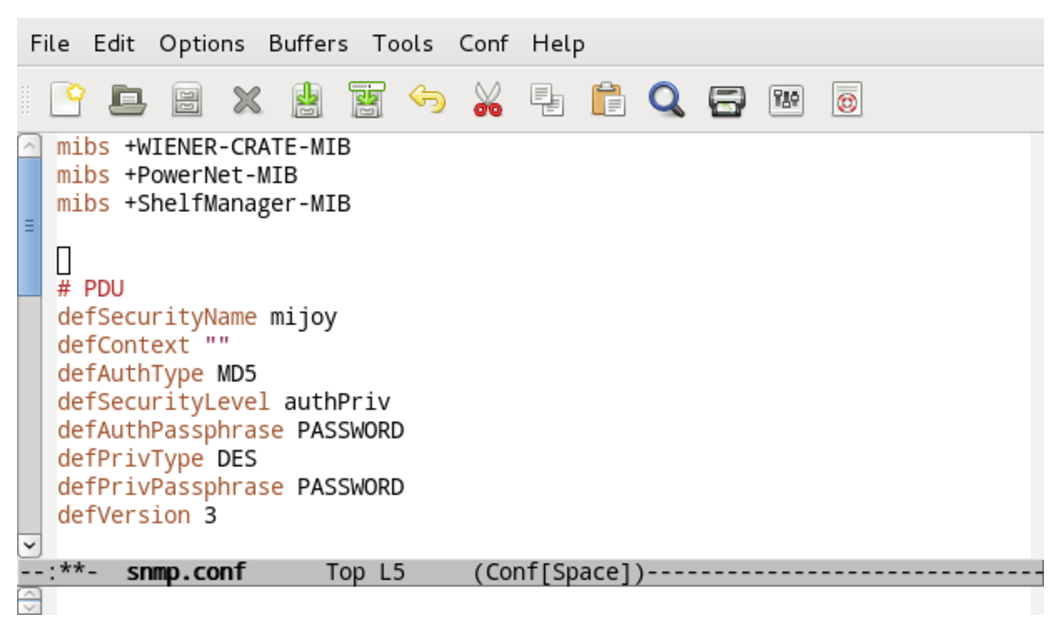
\includegraphics[width=0.99\textwidth]{./images/snmp_conf.eps}
  \caption{snmp.conf 파일}
  \label{fig:snmp_conf}   
\end{figure}

이 외의 SNMP의 추가적인 옵션은 snmpwalk(get...) -h를 이용해 알 수 있다.


\clearpage
\section{장비 모니터링 결과}
SNMP를 이용한 장비 모니터링 결과를 보여주기에 앞서 본 모니터링에 사용된 시스템 및 소프트웨어는 다음과 같다.

\begin{itemize}
\item Debian Linux 7 Wheezy
\item NET-SNMP v5.4.3
\item GNU Bash script-CLI(Command-line Interface) 
\end{itemize}

또한 장비 모니터링에 사용된 장비들과 각 장비들이 지원하는 SNMP버전은 표 \ref{table:used_version}와 같다.

\begin{table}[h]
\begin{center}
\begin{tabular}{c|c}\hline
Device Name & Supported Versions \\ \hline
Printer(Xerox, Kyocera) & v1* (R) \\ \hline
WIENER VME CRATE & v1/2c* (R/W) \\ \hline
ELMA VME CRATE & v3* (R) \\ \hline
APC PDU 7921 & v1/2c/3* (R/W) \\ \hline
\end{tabular}
\caption{연구에 사용된 장비와 SNMP 버전 (R: Read, W: Write / *: 연구에 사용된 버전)}
  \label{table:used_version}  
\end{center}
\end{table} 

\clearpage
\subsection{·프린터}

Xerox사와 Kyocera사의 프린터들에 설정되어 있는 SNMP Agent의 기본 설정을 사용하여 프린터들의 상태를 SNMP로 모니터링(Read) 해보았다. SNMPv1(Read)로 프린터 상태를 모니터링 한 결과로 프린터의 현재 상태, 용지의 종류와 양, 잉크의 잔여량 등의 정보를 알 수 있다.

\begin{lstlisting}[style=termstyle, caption=Printer 모니터링 및 제어결과]]
mijoy0909@mjpark:~/users/mijoy0909$ ./snmptest.sh 
 
Mon Nov 17 10:35:17 KST 2014
 
++++++++++++++++ Printer Status ++++++++++++++++
- 182 Printer              -, "Printing..." "" ""
- 184 Printer              -, "Sleeping " " "
 
++++++++ 182 Printer Paper Current Level ++++++++
- Tray1                    -, 25.000%
- Tray2                    -, 0%
- Tray3                    -, 75.000%
- Tray4                    -, 75.000%
- Tray5                    -, 0%
 
++++++++ 182 Printer Paper Current size ++++++++
- Tray1                    -, A4
- Tray2                    -, A4
- Tray3                    -, A4
- Tray4                    -, A3
- Tray5                    -, -
 
++++++++ 184 Printer Paper Current Level ++++++++
- MP Tray                  -, 0%
- Tray1                    -, 50.000%
- Tray2                    -, 0%
- Tray3                    -, 50.000%
- Tray4                    -, 50.000%
 
++++++++ 184 Printer Paper Current size ++++++++
- MP Tray                  -, A4
- Tray1                    -, A4
- Tray2                    -, -
- Tray3                    -, A3
- Tray4                    -, A3
 
++++++++ 182 Printer Toner Current Level ++++++++
- black                    -, 97.000%
- yellow                   -, 6.000%
- magenta                  -, 9.000%
- cyan                     -, 40.000%
 
++++++++ 184 Printer Toner Current Level ++++++++
- black                    -, 73.000%
 
+++++++++ 182 Printer Printed Page(s) ++++++++++
- total                    -, 477124
 
+++++++++ 184 Printer Printed Page(s) ++++++++++
- total                    -, 86618
\end{lstlisting}


\subsection{·VMEbus Crate(Elma와 Wiener)}
VMEbus Crate들은 가속기를 제어하는데 있어 중요한 장비들이며, 가속기 시설의 특성상 즉각적인 접근이 불가능한 지역에 설치되는 경우가 많다. 이러한 이유로 다른 장비들과 다르게 쓰기(Write)권한이 필요하며, 신호의 보안에도 신경을 써야한다. 이번 실험에서는 Elma제품은 v3(Read)로, Wiener제품은 현재 지원하는 v2c로 테스트를 진행하였다. Wiener, Elma사의 VMEbus Crate는 그림 \ref{fig:elmawiener}이다.


\begin{figure}[h]
  \centering
  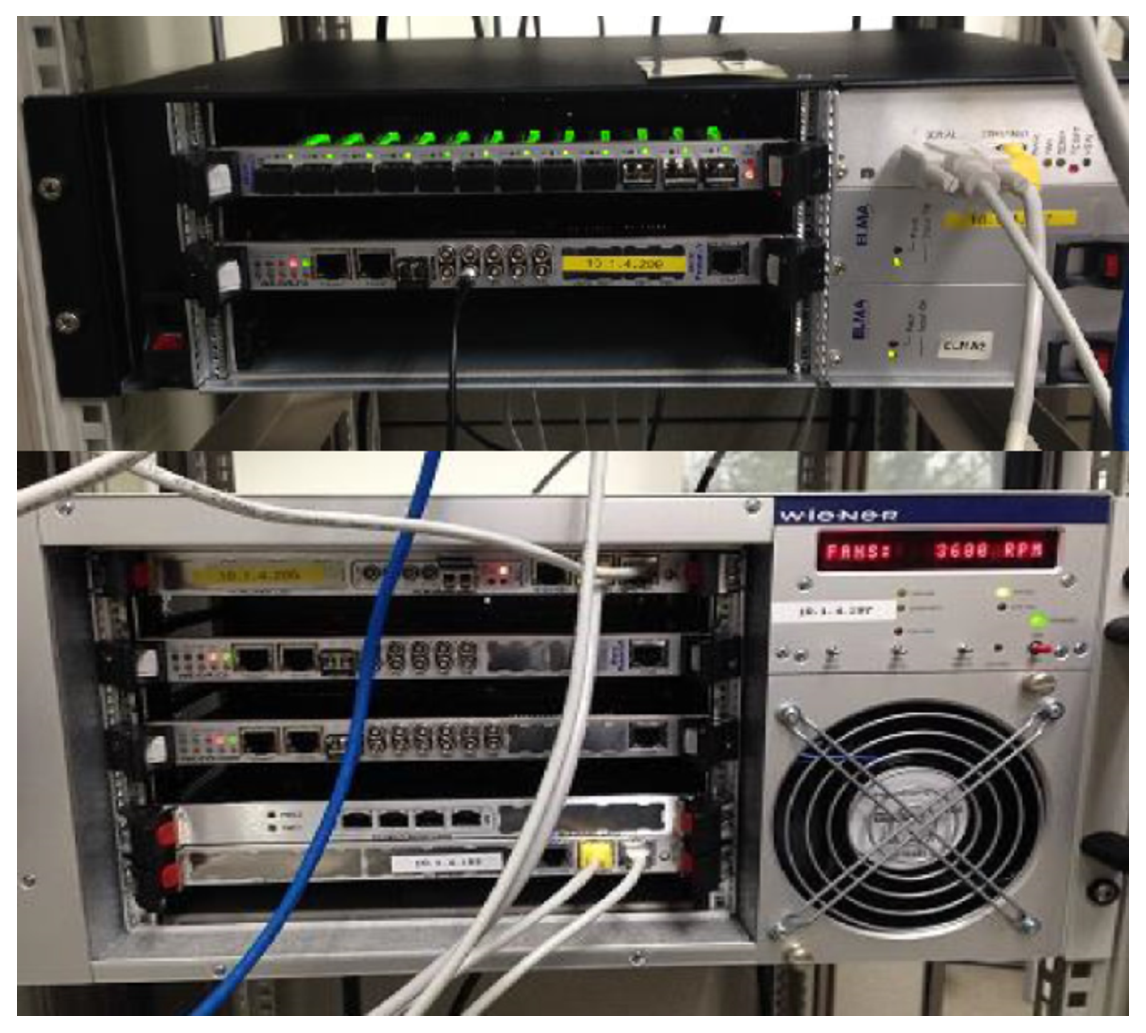
\includegraphics[width=0.7\textwidth]{./images/elmawiener.eps}
  \caption{ELMA, WIENER Crate (위 : ELMA, 아래: WIENER)}
  \label{fig:elmawiener}   
\end{figure}

\vspace{2mm}

Wiener사의 Crate는 Crate의 상태, 팬 스피드, 온도 등에 대한 모니터링(Read)뿐만 아니라 메인 스위치의 동작과 팬 스피드를 제어(Write)하는 테스트를 수행하였고, Elma Crate는 Crate 상태, 온도 등을 모니터링했다. Elma사는 Crate의 개별 실험 결과는 다음와 같다.

\vspace{5cm}
- ELMA
\begin{lstlisting}[style=termstyle, caption=ELMA Crate 모니터링 및 제어결과]]
mijoy0909@mjpark:~/users/mijoy0909$ ./elma_test1.sh

- Voltage
==================================================
   #         Name          Value          State
==================================================
   1     "+3.3V"          3.290 V          OK
   2       "+5V"          4.980 V          OK
   3      "+12V"         11.960 V          OK
   4      "-12V"    2147483.647 V          OK
==================================================

- Temp
==================================================
   #         Name          Value          State
==================================================
   1       "Temp 1"       37 deg C         OK
   2       "Temp 2"       27 deg C         OK
   3       "Temp 3"       24 deg C         OK
==================================================

- Fan
==================================================
   #         Name          Value          State
==================================================
   1        "Fan 1"       3400 RPM         OK
   2        "Fan 2"       3400 RPM         OK
   3        "Fan 3"       3400 RPM         OK
   4        "Fan 4"       3400 RPM         OK
   5        "Fan 5"       3500 RPM         OK
   6        "Fan 6"       3400 RPM         OK
==================================================
\end{lstlisting}

\vspace{5mm}
- WIENER
\begin{lstlisting}[style=termstyle, caption=Wiener Crate 모니터링 및 제어결과]]
***************************************
*               OPTIONS               *
***************************************
  [s] Status                           
  [1] Main Switch ON/OFF               
  [2] Change Fan Speed (1200~3600 RPM) 
  [q] Exit                             
  [0] Help                             
***************************************
-> Please enter your choice : 2

- Main Switch : ON
- Fan Speed : 3500 RPM
- Temperature Sensors1 : 25 deg C
- Temperature Sensors2 : 22 deg C

- Voltage
========================================
 Name        Value          State
========================================
  U0         3.33 V           On
  U1         5.01 V           On
  U2        12.06 V           On
  U3       -12.24 V           On
========================================

Enter Fan Speed (0~3600 RPM) : 
3600
INTEGER: 3600 RPM

- Main Switch : ON
- Fan Speed : 3600 RPM
- Temperature Sensors1 : 25 deg C
- Temperature Sensors2 : 22 deg C
\end{lstlisting}


\subsection{·Power Distribution Unit}
VMEbus Crate처럼 모니터링(Read) 및 제어(Write)가 가능해야하는 Power supply는 모든 버전의 SNMP를 지원하는 APC사의 Power Distribution Unit (PDU) 7921(그림 \ref{fig:apc_pdu})을 이용하여, v3에서 읽기와 쓰기에 필요한 여러 설정을 테스트 해볼 수 있었다. 아래는 SNMPv3를 통해 APC PDU를 모니터링(Read) 및 제어(Write)의 결과이다. 장비의 상태, 사용전력, 부하된 전류량 등을 모니터링 할 수 있으며, 장비에서 지원하는 다양한 옵션으로 각각의 power outlet을 제어 할 수 있다.

\begin{figure}[h]
  \centering
  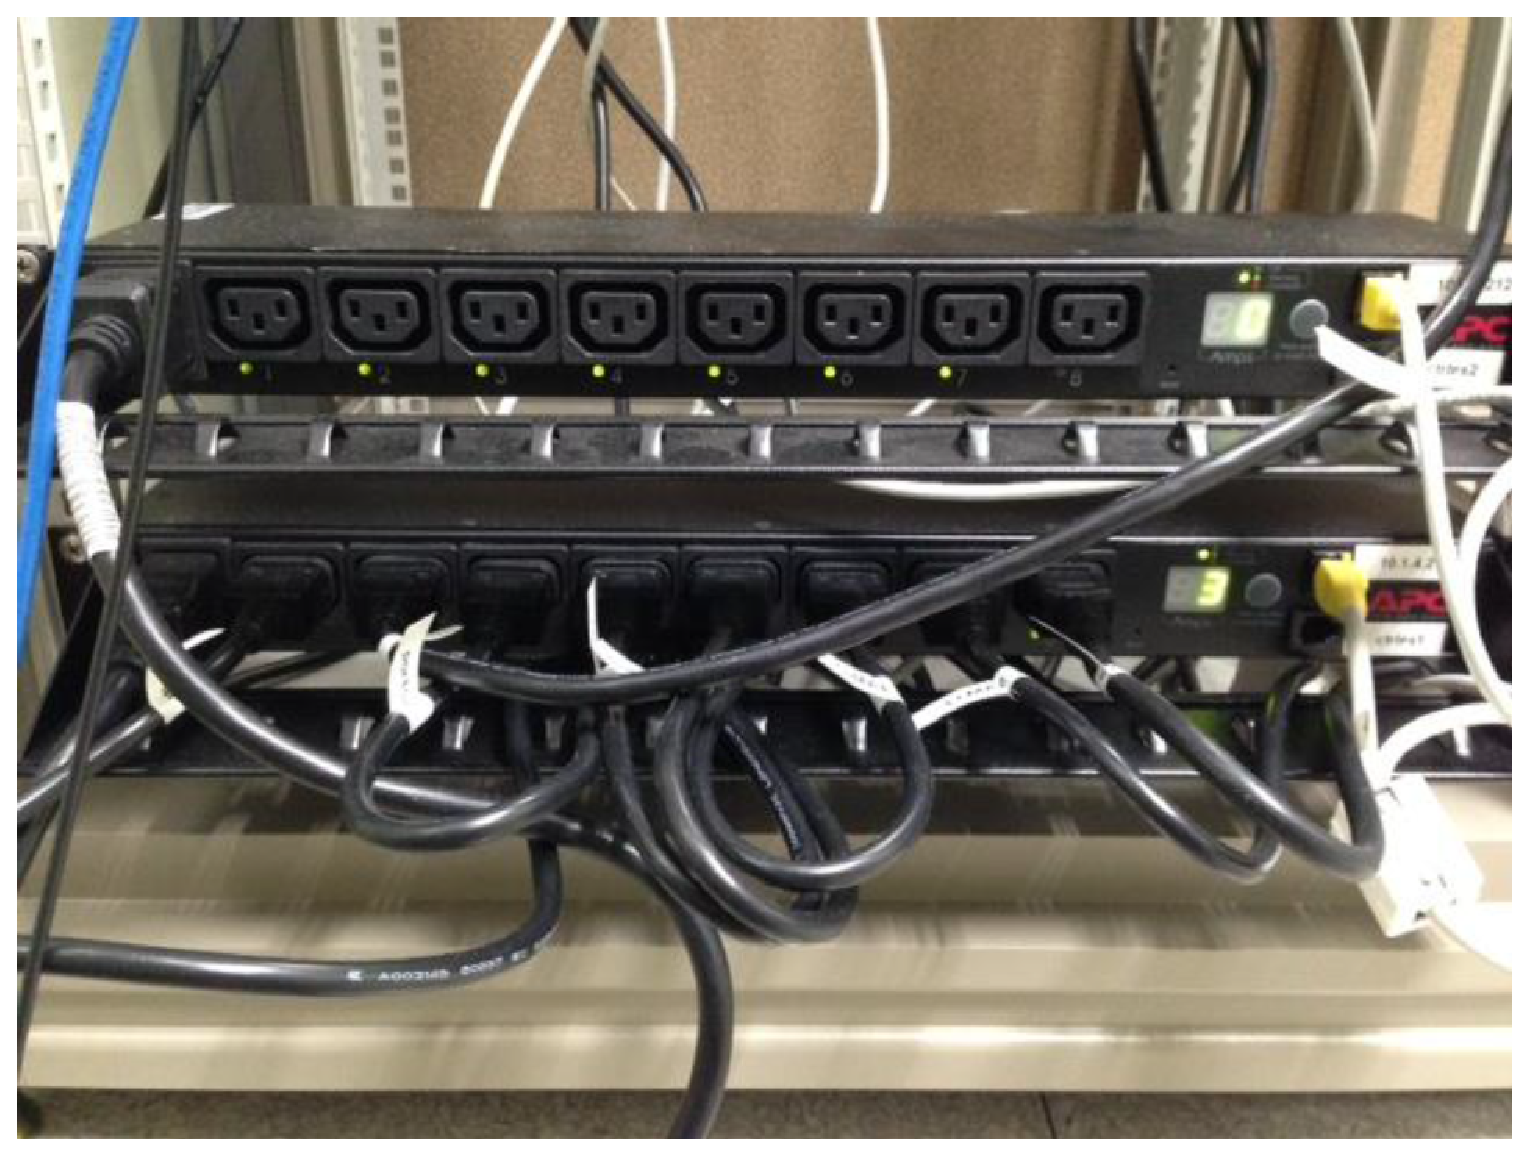
\includegraphics[width=0.6\textwidth]{./images/apc_pdu.eps}
  \caption{APC PDU}
  \label{fig:apc_pdu}   
\end{figure}

\begin{lstlisting}[style=termstyle, caption=APC PDU 모니터링 및 제어결과]]
mijoy0909@mjpark:~/users/mijoy0909$ ./powernet_test8.sh

*****************************
*          OPTIONS          *
*****************************
  [s] Status                 
  [1] ON                     
  [2] OFF                    
  [3] Reboot                 
  [4] On with delay          
  [5] Off with delay         
  [6] Reboot with delay      
  [q] Exit                   
  [0] Help                   
*****************************
-> Please enter your choice : 2

------------------------------------------------------------

 PowerWatts                      , 220
 Load Status                     , 1.0 Amps

   #       Name       Status      Control Outlet Command
============================================================
   1     "Outlet 1"      On              immediateOn
   2     "Outlet 2"      On              immediateOn
   3     "Outlet 3"      On              immediateOn
   4     "Outlet 4"      On              immediateOn
   5     "Outlet 5"      On              immediateOn
   6     "Outlet 6"      On              immediateOn
   7     "Outlet 7"      On              immediateOn
   8     "Outlet 8"      On              immediateOn
============================================================
------------------------------------------------------------

  [s] Status                 
  [1] Outlet1                
  [2] Outlet2                
  [3] Outlet3                
  [4] Outlet4                
  [5] Outlet5                
  [6] Outlet6                
  [7] Outlet7                
  [8] Outlet8                
  [b] Back                   
  [q] Exit                   
  [0] Help                   
-> Select outlet: 8
-> Are you sure? [y/n]y
outletOff

------------------------------------------------------------

 PowerWatts                      , 220
 Load Status                     , 1.0 Amps

   #       Name       Status      Control Outlet Command
============================================================
   1     "Outlet 1"      On              immediateOn
   2     "Outlet 2"      On              immediateOn
   3     "Outlet 3"      On              immediateOn
   4     "Outlet 4"      On              immediateOn
   5     "Outlet 5"      On              immediateOn
   6     "Outlet 6"      On              immediateOn
   7     "Outlet 7"      On              immediateOn
   8     "Outlet 8"     Off             immediateOff
============================================================
------------------------------------------------------------
\end{lstlisting}


\clearpage

\chapter{SNMP 응답시간 테스트}

가속기 제어 시스템에서 시설의 복잡성과 장비의 다양성, 그리고 안전한 장비 접근성을 만족하며, 동시에 장비의 안정된 응답시간을 만족시키는 설치위치를 선정하는 것은 어렵기 때문에 장비의 응답시간을 고려하여 제어 네트워크 토폴로지 설계 및 네트워크 보안에 따른 SNMP의 응답시간 최적화 설계가 필요하다. 따라서 실험 당시 SNMP의 모든 버전(v1/2c/3)을 지원하는 장비인 APC PDU 7921을 사용하여 모니터링 및 제어를 하는데 걸리는 응답시간에 대한 테스트를 진행했다.

\begin{table}[h!]
\begin{center}
\begin{tabular}{c|c|c|c|c}\hline
 & v1 & v2c & v3(r) & v3(w) \\ \hline
mean & 2.863 & 2.852 & 4.101 & 4.138 \\ \hline
sample deviation & 0.867 & 0.840 & 0.814 & 0.864 \\ \hline
\end{tabular}
\caption{SNMP 버전에 따른 응답시간(wall-clock time response)의 차이 (단위: ms)}
  \label{table:test}  
\end{center}
\end{table}

표 \ref{table:test}은 버전별 응답시간을 측정한 결과이다. 이 테스트에서는 암호화 및 복호화에 걸리는 시간, 케이블 딜레이, 하드웨어 자체의 속도 및 사용된 Linux OS에 대한 응답시간 차이가 동일하다는 가정을 하였다. 이러한 가정 하에서 SNMPv1/2c는 서로 비교할 수 없는 오차 범위에 있으며, v3는 읽기(R)와 쓰기(W)에서 타 버전에 비해 1.5배 정도의 시간이 더 소모됨을 확인 할 수 있다.

\section{실험 목적}
앞서 언급했듯이 장비의 응답시간은 제어 네트워크에서 중요하다. 가속기 제어 네트워크 토폴로지 설계에 필요한 물리적인 구성요소는 Layer 2 스위치와 UTP 케이블의 길이이므로 이러한 요소들로 토폴로지 내에서 가능하고, 이상적인 장비의 응답시간과 구성요소들 간의 상관관계를 측정하는 것이 필요하다. 이렇게 측정된 결과들은 네트워크 토폴로지 설계 및 장비의 최적화된 설치위치 선정에 도움이 될 것이다.

\section{실험 방법}
본 실험에서는 프로그램이 수행되는 시간을 측정하는 리눅스의 time 명령어를 이용하여 SNMP명령어를 1000번 수행한 시간을 응답시간으로 측정하였다. time 명령어는 세 가지 다른 형태의 시간 측정 결과를 나타낸다. 실제로 얼마만큼의 시간이 걸렸는가 하는 real, 커널이 사용한 시간을 제외하고 CPU에서 소비된 시간을 나타내는 user, 그리고 실제로 얼마만큼의 커널 시간을 할애했는가 하는 sys시간이 있다. user+sys의 시간은 실제로 작업에 할애된 시간이며, real-(user+sys)의 시
간은 다른 프로세서 처리에 할당된 시간이다\citep{time_command}. 
본 실험에서는 실제 작업시간인 user+sys시간을 사용한다. 이는 Layer 2 스위치 간의 내부 시간 차이와 케이블을 제작하는 중 발생하는 길이의 오차 등에서 발생하는 시간이 포함된 것이다. UTP케이블이 물리적으로 신호를 안정적으로 전달할 수 있는 최대 길이가 100m이기 때문에 본 실험에는 1m, 10m, 20m, 30m, 40m, 50m, 100m 길이의 CAT6 LAN 케이블을 사용하였다.
실험에 사용된 시스템 및 소프트웨어는 다음과 같다.

\begin{itemize}
\item Debian Linux 7 Wheezy
\item NET-SNMP v5.4.3
\item R v2.15.1
\item GNU Bash script-CLI(Command-line Interface) 
\item Switch(BROCADE ICX6430)
\item Power Distribution Unit(APC PDU 7921)
\end{itemize}

\begin{lstlisting}[style=termstyle, caption=GNU Bash script를 통한 CLI]
mijoy0909@mjpark:~/speedtest$ ./speedtest.sh 

**********************************
*               OPTIONS          *
**********************************
  [1] SNMP Speed Test             
  [2] File Merge                  
  [3] R(Linear)                   
  [4] R(Histogram)                
----------------------------------
----------------------------------
  [5] Edit R(linear)              
  [6] Edit R(histogram)           
----------------------------------
----------------------------------
  [q] Exit                        
  [0] Help                        
**********************************
-> Select sub option: 1


****************************************
*              SUB OPTIONS             *
****************************************
  [1] SNMP v1        / sleep x          
  [2] SNMP v1        / sleep 1          
  [3] SNMP v2c       / sleep x          
  [4] SNMP v2c       / sleep 1          
  [5] SNMP v3(read)  / sleep x          
  [6] SNMP v3(read)  / sleep 1          
  [7] SNMP v3(write) / sleep x          
  [8] SNMP v3(write) / sleep 1          
  [b] Back                              
  [q] Exit                              
  [0] Help                              
***************************************
-> Select sub option: 1

Enter name you wish to save [ex.example] :S1V1SXC1
/home/mijoy0909/speedtest
outletOn
outletOn
.
outletOn
-----------------------------------------------
<real>

Total count        :       1000
Mean               : 0.09147000
Sample Deviation   : 0.00503631
Standard Deviation : 0.00503380

-----------------------------------------------
<user>

Total count        :       1000
Mean               : 0.06384000
Sample Deviation   : 0.00590672
Standard Deviation : 0.00590376

-----------------------------------------------
<sys>

Total count        :       1000
Mean               : 0.00061000
Sample Deviation   : 0.00247670
Standard Deviation : 0.00247546

***********************************************

Mean(user+sys)             : 0.03222500
Sample Deviation(user+sys) : 0.00640495

***********************************************
-----------------------------------------------
\end{lstlisting}

SNMPv1/2c/3의 응답시간 측정에는 GNU Bash를 이용하여 만든 script를 사용한다. 이 script는 지정한 시간동안 시스템을 멈추는 sleep 명령어를 사용해 시스템을 1초 멈추는 조건과 sleep을 사용하지 않는 조건으로 SNMPGET, SET 명령어를 1000번 보내고 응답받는 시간을 time 명령어의 user+sys시간으로 측정 , CLI로 total count, mean, sample deviation, standard deviation의 측정 결과를 보여준다.

\begin{figure}[!htb]
  \centering
  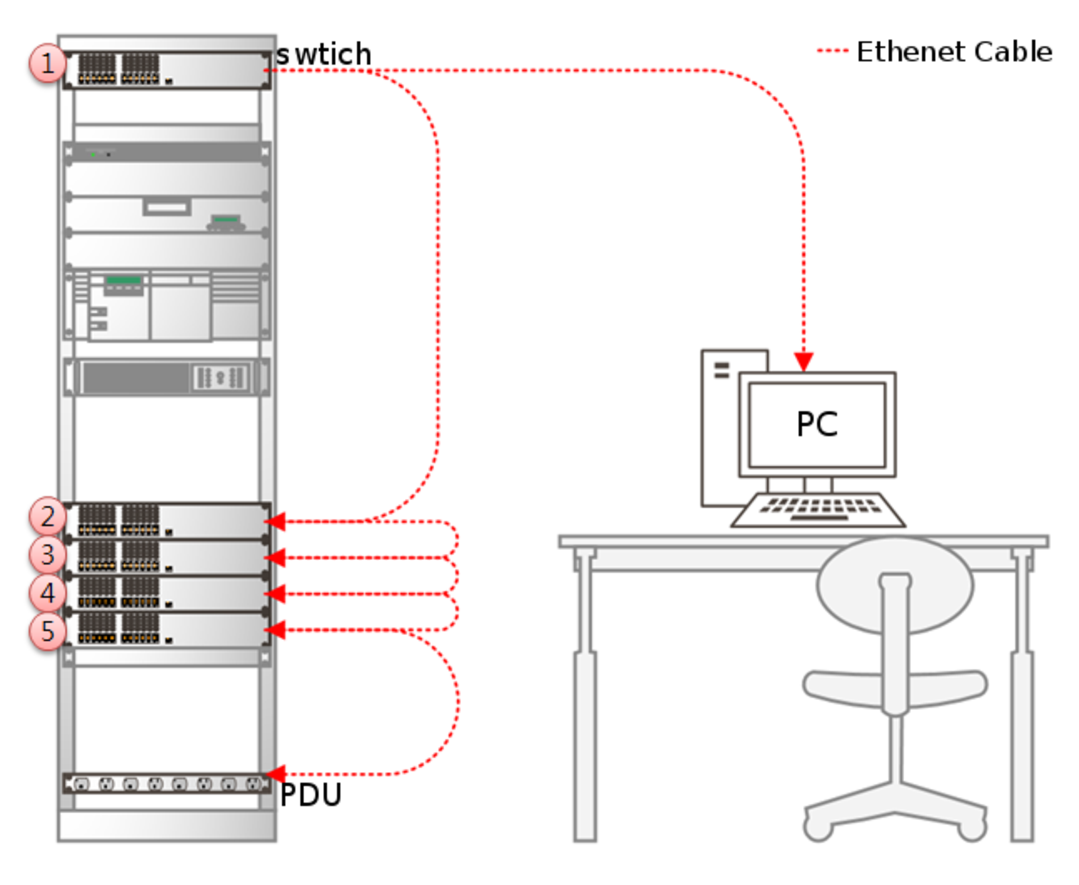
\includegraphics[width=0.4\textwidth]{./images/switch5.eps}
  \caption{테스트 배치}
  \label{fig:switch}   
\end{figure}

그림  \ref{fig:switch}은 스위치 5개를 연결 했을 때의 실험 배치도이다. 길이가 1m인 케이블을 이용하여 응답시간을 측정하고자 할 때, 컴퓨터, PDU, 스위치를 네트워크 케이블로 연결한 후 script를 실행하여 응답시간을 측정한다. 이 후 1m 케이블로 스위치의 개수를 증가시키면서 테스트를 진행한다. 이 때, 컴퓨터는 첫 번째 스위치에 계속해 연결되어있고, 스위치의 개수를 5개까지 추가하면서 마지막 스위치에 PDU를 연결한다. 다른 길이의 케이블도 각각 위의 과정을 테스트한다. 

\begin{figure}[!htb]
  \centering
  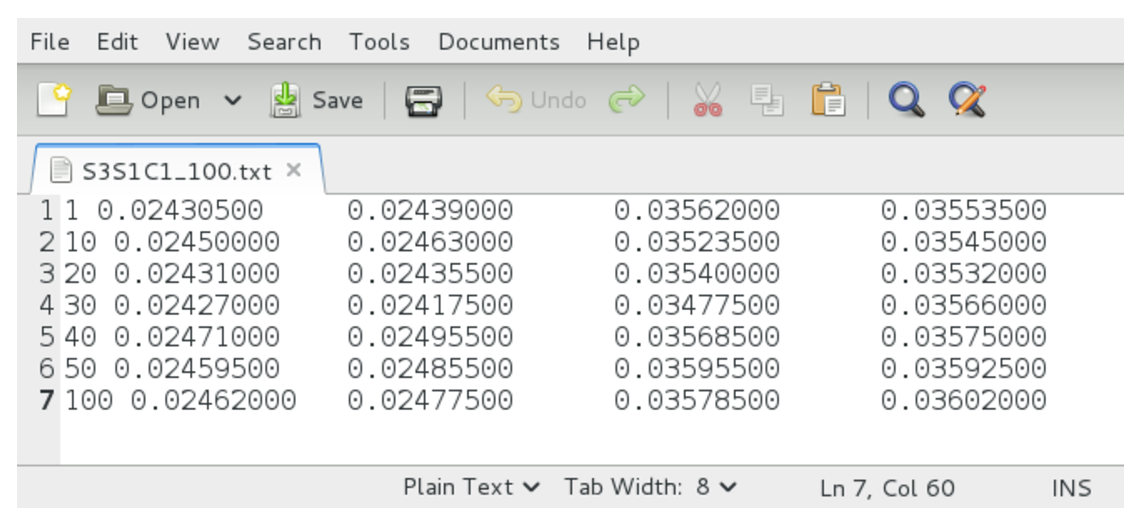
\includegraphics[width=0.7\textwidth]{./images/timetable.eps}
  \caption{데이터 테이블}
  \label{fig:time_table}   
\end{figure}

이렇게 측정된 응답시간의 mean값은 ASCII 파일로 저장이 되고, 이 ASCII 파일은 그림 \ref{fig:time_table}와 같이 데이터 테이블로 재구성된다. 이렇게 만들어진 데이터 테이블을 이용해 통계 계산과 그래픽을 위한 프로그래밍 언어이자 소프트웨어 환경인 R\citep{r}을 통해 통계적 예측과 분석을 수행한다. 

\clearpage
\section{실험 결과}
\subsection{3.3.1 R을 이용한 통계적 데이터 분석}

통계적 분석에 앞서 본 연구에서는 케이블 길이가 길어질수록 응답시간이 클 것이라는 가설을 세웠고, 두 변수간의 관련성을 연구할 만한 자료인지 판단하기 위해 산점도와 linear fitting을 통한 linear그래프를 두 그려 두 변수의 상관관계를 확인하였다. 그림 \ref{fig:linear}은 스위치의 개수와 SNMP 버전에서의 케이블길이와 응답시간에 대한 그래프이다. 대부분의 그래프에서 케이블의 길이가 길어질수록 응답시간이 크다는 것을 알 수 있다.

\begin{figure}[!htb]
  \centering
  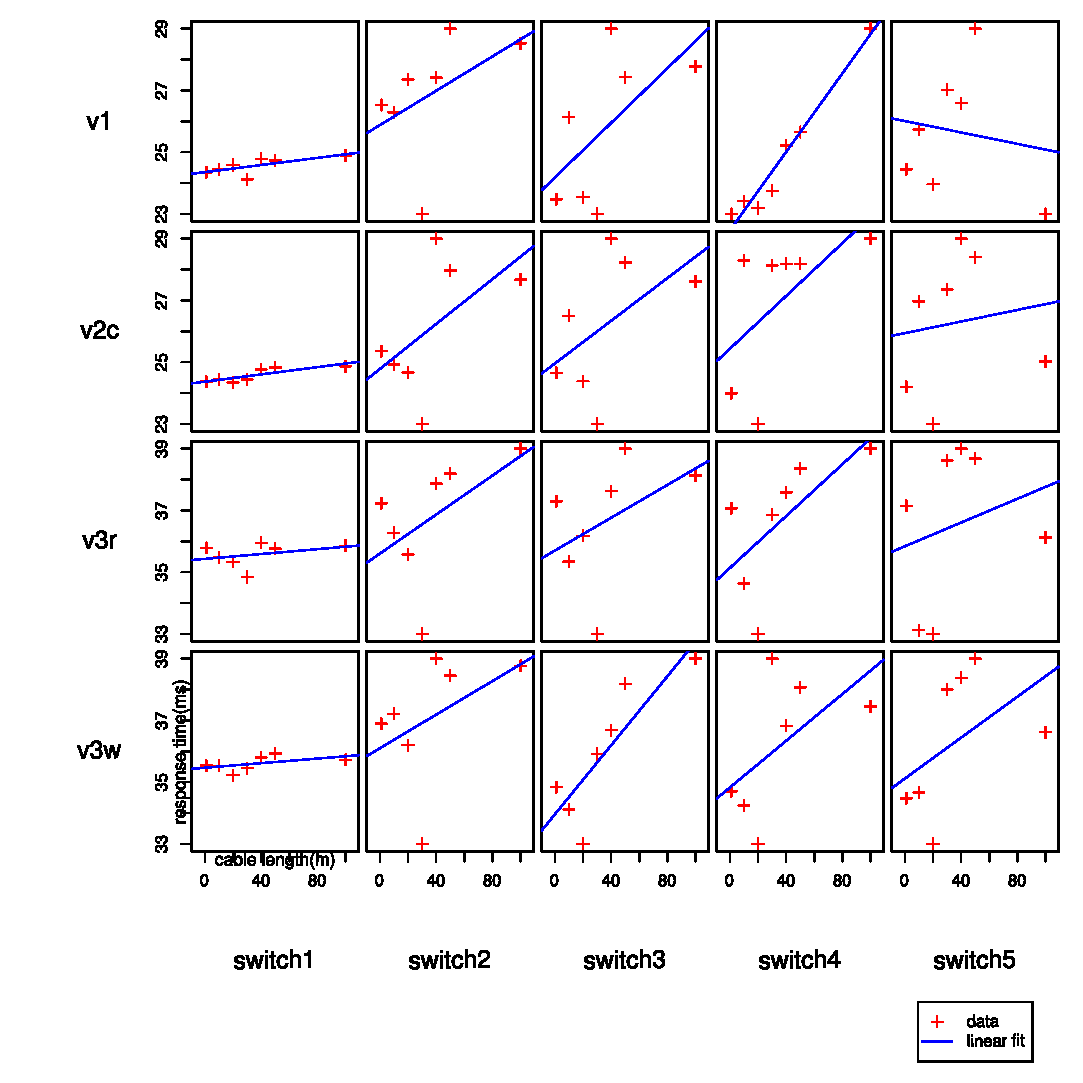
\includegraphics[width=0.9\textwidth]{./images/sleep1_switch.eps}
  \caption{산점도와 linear 그래프}
  \label{fig:linear}   
\end{figure}

\clearpage

\subsection{3.3.2 회귀분석을 통한 분석 및 예측}

본 연구에서는 하나 또는 그 이상의 독립변수(x)의 종속변수(y)에 대한 영향의 추정을 할 수 있는 통계기법인 회귀분석을 사용하여 데이터를 분석하였다\citep{analysis}. 회귀분석에서 독립변수는 다른 변수에 영향을 미치는 변수이고, 종속변수는 독립변수에 의해 영향을 받는 변수이다. 따라서 본 연구에서의 독립변수는 케이블 길이이고, 종속변수는 응답시간이다. 회귀분석은 최소 하나 이상의 독립변수의 값에 근거하여 종속변수의 값을 예측하거나 독립변수가 종속변수에 미치는 영향력의 크기를 설명하는데 유용하다. 종속변수가 독립변수에 어떻게 관련되어 있는가를 나타내는 방정식은 회귀모델이며, 실험의 회귀모델은 식(1)과 같다. 

y=α+βx         ······(1)

그림 \ref{fig:s3s1}은 스위치가 세개 연결되었을 때 SNMPv2c와 v3w의 네트워크 케이블 길이에 따른 응답시간에 대한 단순회귀분석그래프이다. 

\begin{figure}[!htb]
  \centering
  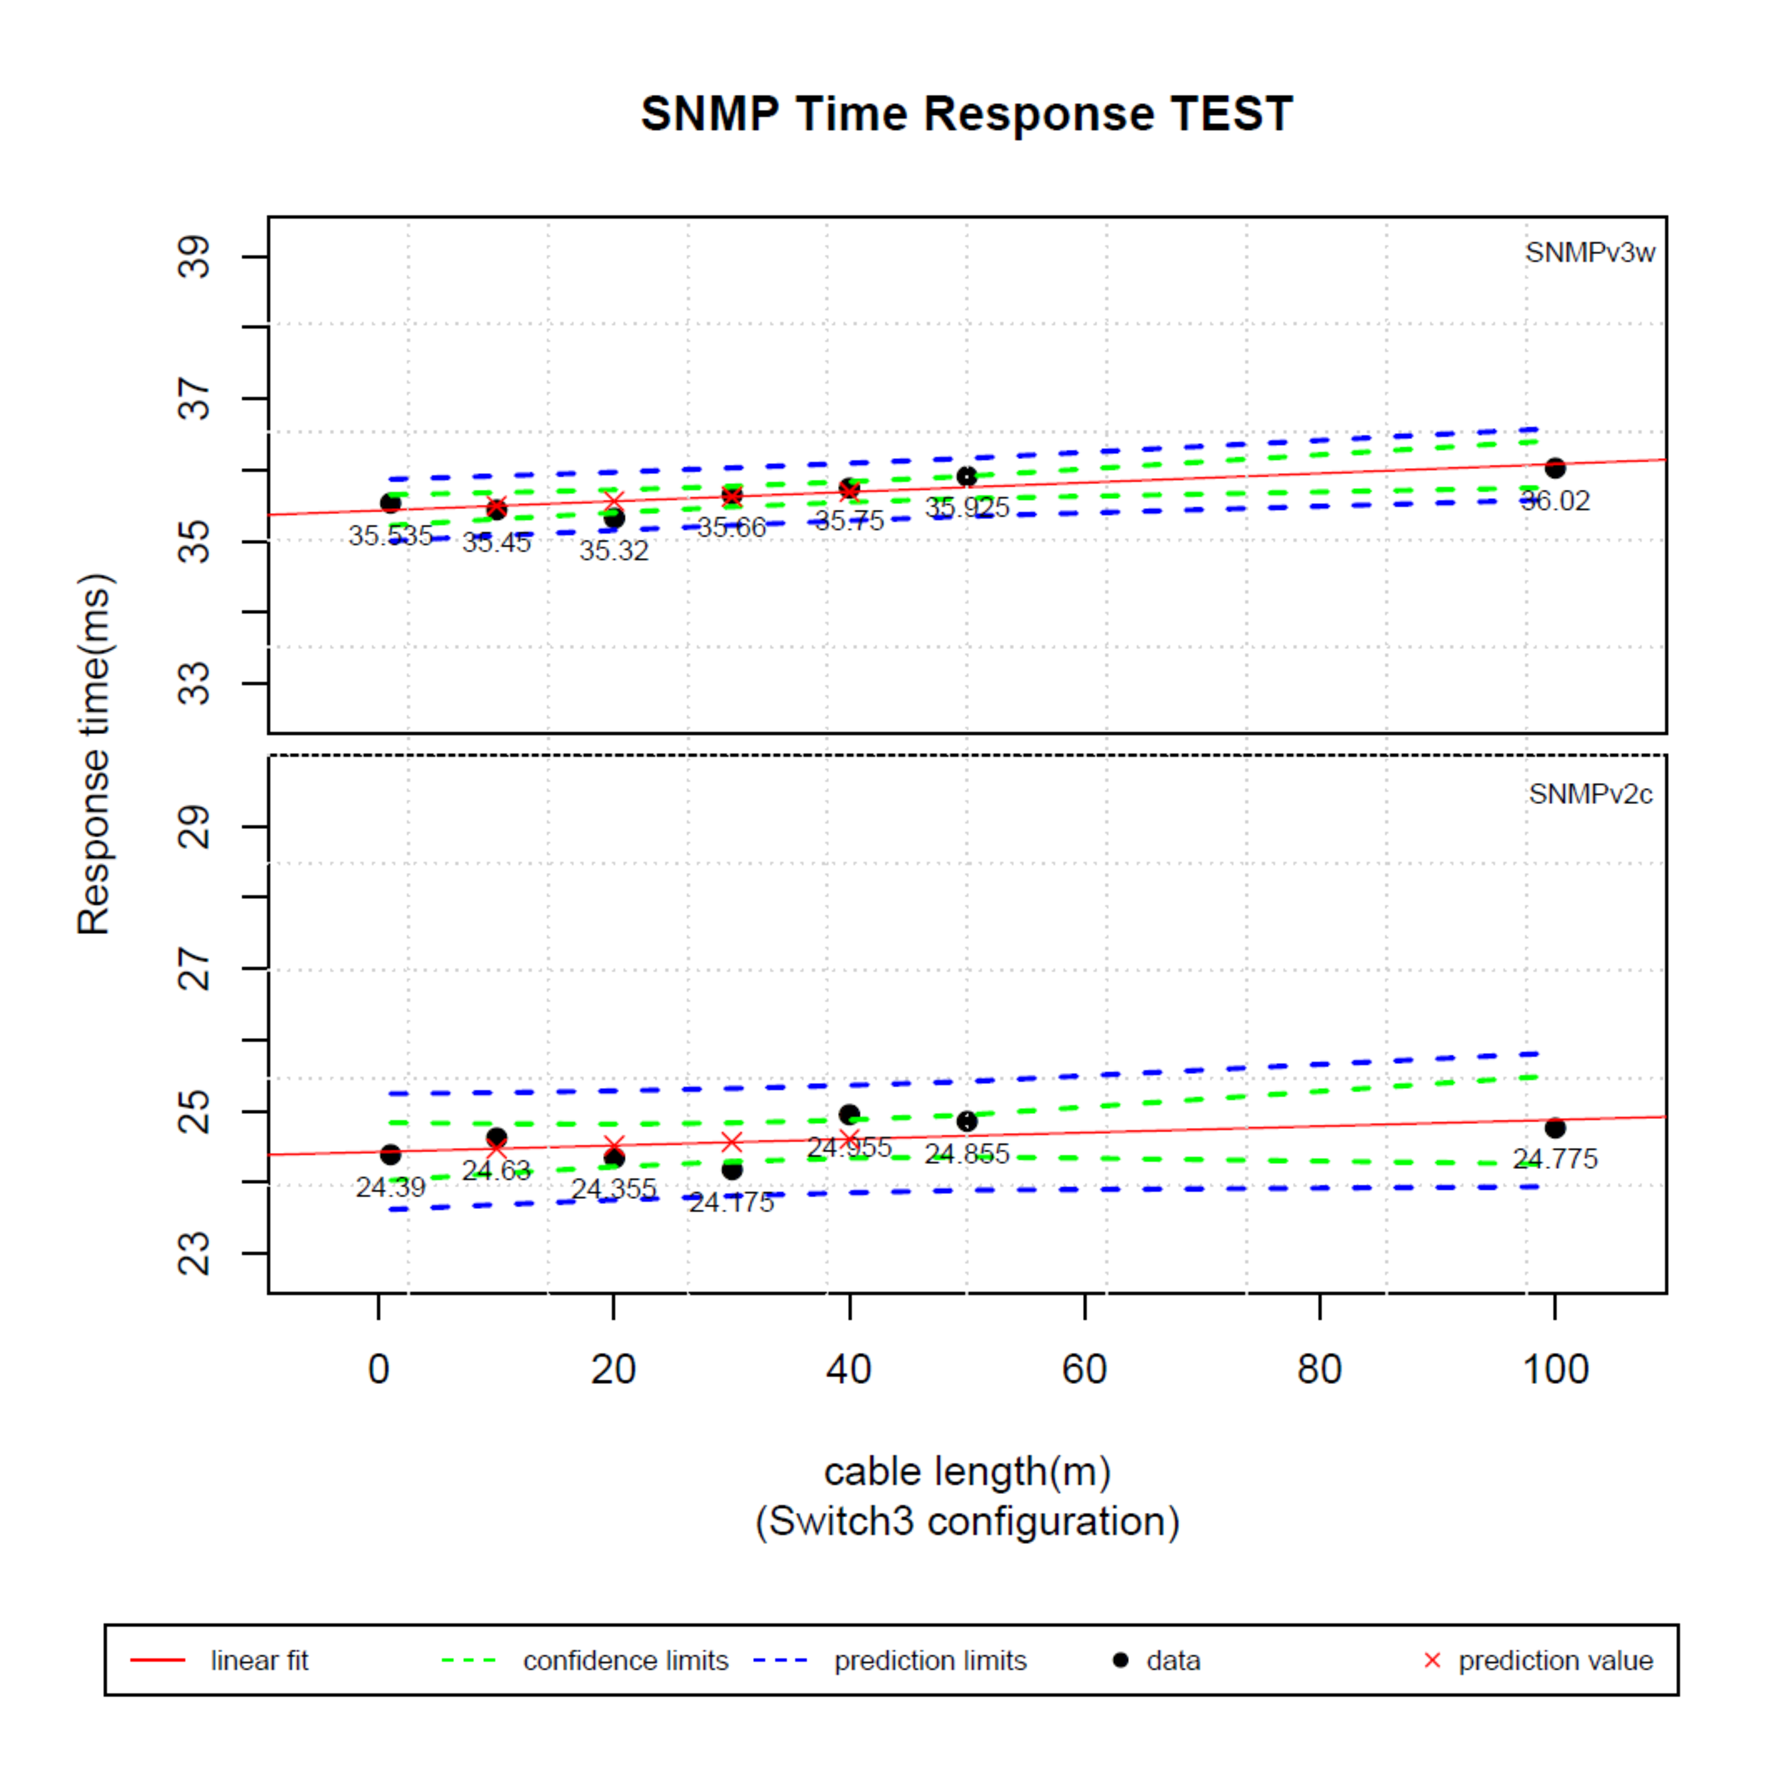
\includegraphics[width=0.9\textwidth]{./images/s3s1.eps}
  \caption{회귀분석 그래프 스위치 3개/Sleep1}
  \label{fig:s3s1}   
\end{figure}

여기서 confidence limit(녹색점선)은 추가적으로 실험을 진행할 때 1, 10, 20, 30, 40, 50, 100m 길이에서 나올 수 있는 응답시간의 범위를 나타내고, prediction limit(청색점선)은 1, 10, 20, 30, 40, 50, 100m의 길이가 아닌 길이의 케이블을 사용하여 응답시간을 측정하였을 때 나올 수 있는 응답시간의 범위이다. 그래프에서 ●는 1, 10, 20, 30, 40, 50, 100m의 케이블 길이에서 측정한 데이터 포인터 값이며, ▲는 회귀모델의 피팅을 통해 특정한 네트워크 케이블 10, 20, 30, 40m의 길이에서의 응답시간을 예측한 값이다. 

\begin{table}[h!]
\begin{center}
\begin{tabular}{c|c|c|c|c}\hline
길이(m) & 10 & 20 & 30 & 40 \\ \hline
예측응답시간(ms)& 35.50 & 35.56 & 35.63 & 35.69 \\ \hline
실제응답시간(ms)& 35.45 & 35.32 & 35.75 & 36.02 \\ \hline
\end{tabular}
\caption{케이블 길이에 따른 응답시간}
  \label{table:predict_time}  
\end{center}
\end{table} 

표 \ref{table:predict_time}는 스위치 3개를 연결했을 때 SNMPv3w의 케이블 길이에 따른 응답시간 예측의 결과이다. 
본 실험에서는 네트워크 케이블의 길이가 증가할수록 응답시간이 커질 것이라고 예측하였고, 특정한 네트워크 케이블 길이에서의 응답시간을 예측하였다. 

\begin{table}[h!]
\begin{center}
\begin{tabular}{c|c}\hline
Independent variable & Value  \\ \hline\hline
p-value &  0.0155\\ 
F-value &  13\\ 
R2 &  0.722\\ 
Adjusted R2 & 0.666 \\ \hline
\multicolumn{2}{l}{*p < 0.05} \\ \hline\hline
\end{tabular}
\caption{스위치 3개일 때 SNMPv3w의 회귀분석결과}
  \label{table:regression}  
\end{center}
\end{table} 

표 \ref{table:regression}는 스위치를 세개 연결하였을 때 v3w에서 케이블 길이에 대한 응답시간의 회귀분석결과이다. R2은 종속변수의 총 변동에서 독립변수의 변동에 의해 설명되는 부분이 차지하는 비중을 의미한다. 이 경우에는 응답시간 변동의 약 72.2\%를 케이블 길이 변동에 의해 설명할 수 있다. 또한, p-value가 0.0155로 α인 0.05보다 작으므로 가설이 통계적으로 유의하다고 할 수 있다. 하지만 대부분의 실험의 결과는 가설이 통계적으로 유의하지 않았다(\ref{txt:result}). 이는 측정한 시간이 모두 오차범위 안에 있으며, 또한 실험이 정밀하지 못함에서 이유를 찾을 수 있다. 

\clearpage
\chapter{회귀분석 그래프와 결과}

\section{회귀분석 그래프}

\subsection{4.1.1 스위치 1개}
 \begin{figure}[!htb]
  \centering
  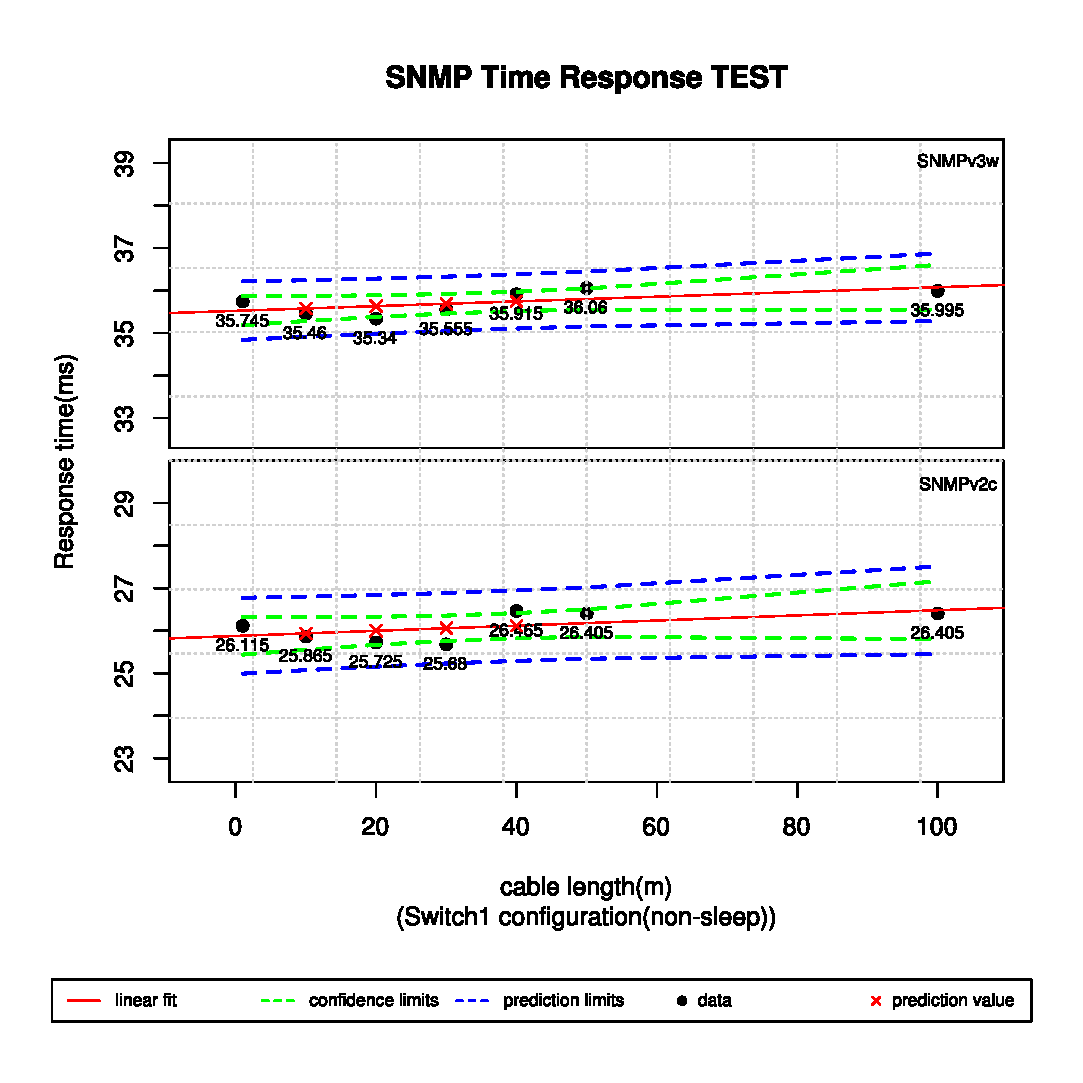
\includegraphics[width=0.5\textwidth]{./images/s1sx.eps}
  \caption{회귀분석 그래프 스위치 1개/Sleepx}
\end{figure}
 \begin{figure}[!htb]
  \centering
  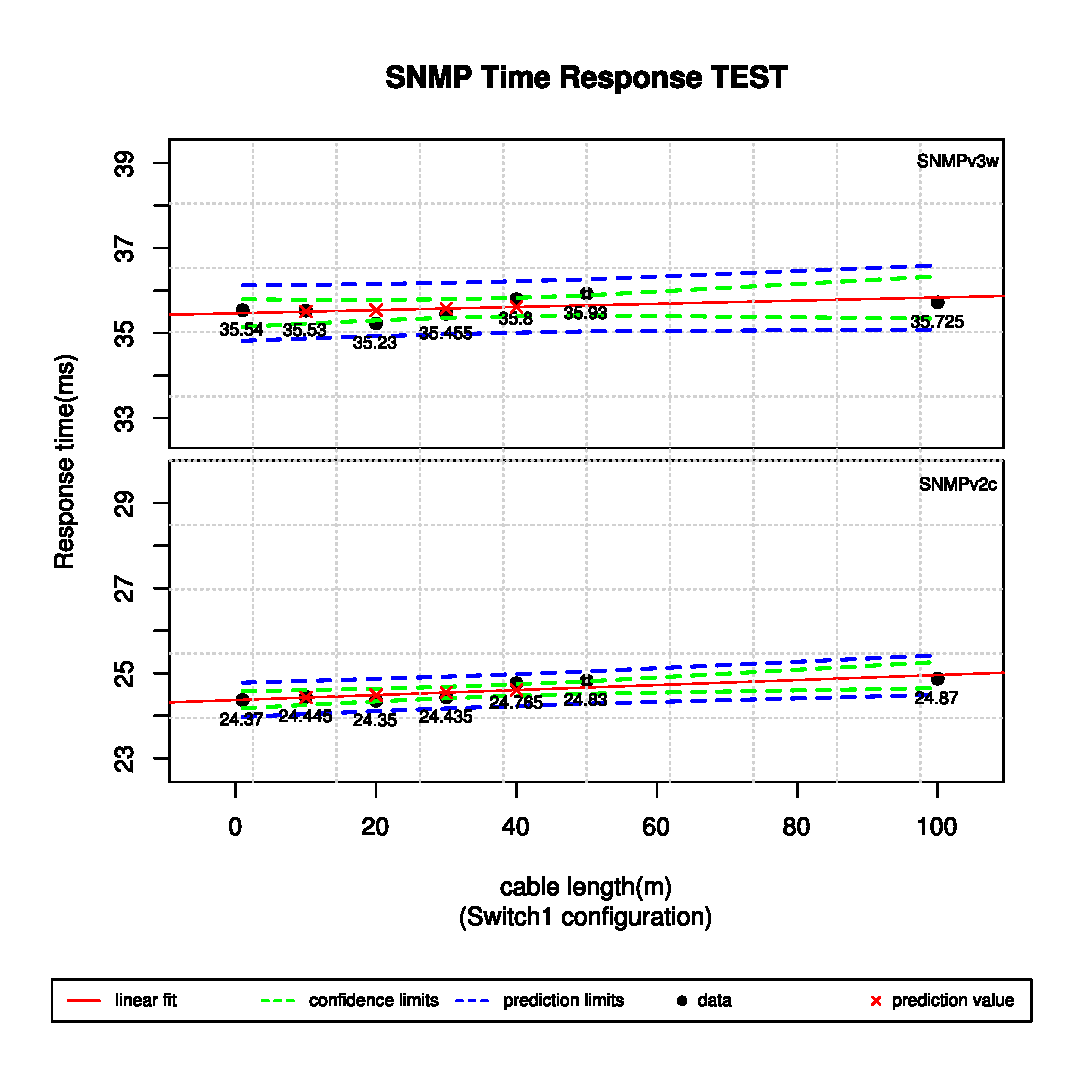
\includegraphics[width=0.5\textwidth]{./images/s1s1.eps}
  \caption{회귀분석 그래프 스위치 1개/Sleep1}
\end{figure}

\clearpage

\subsection{4.1.2 스위치 2개}
 \begin{figure}[!htb]
  \centering
  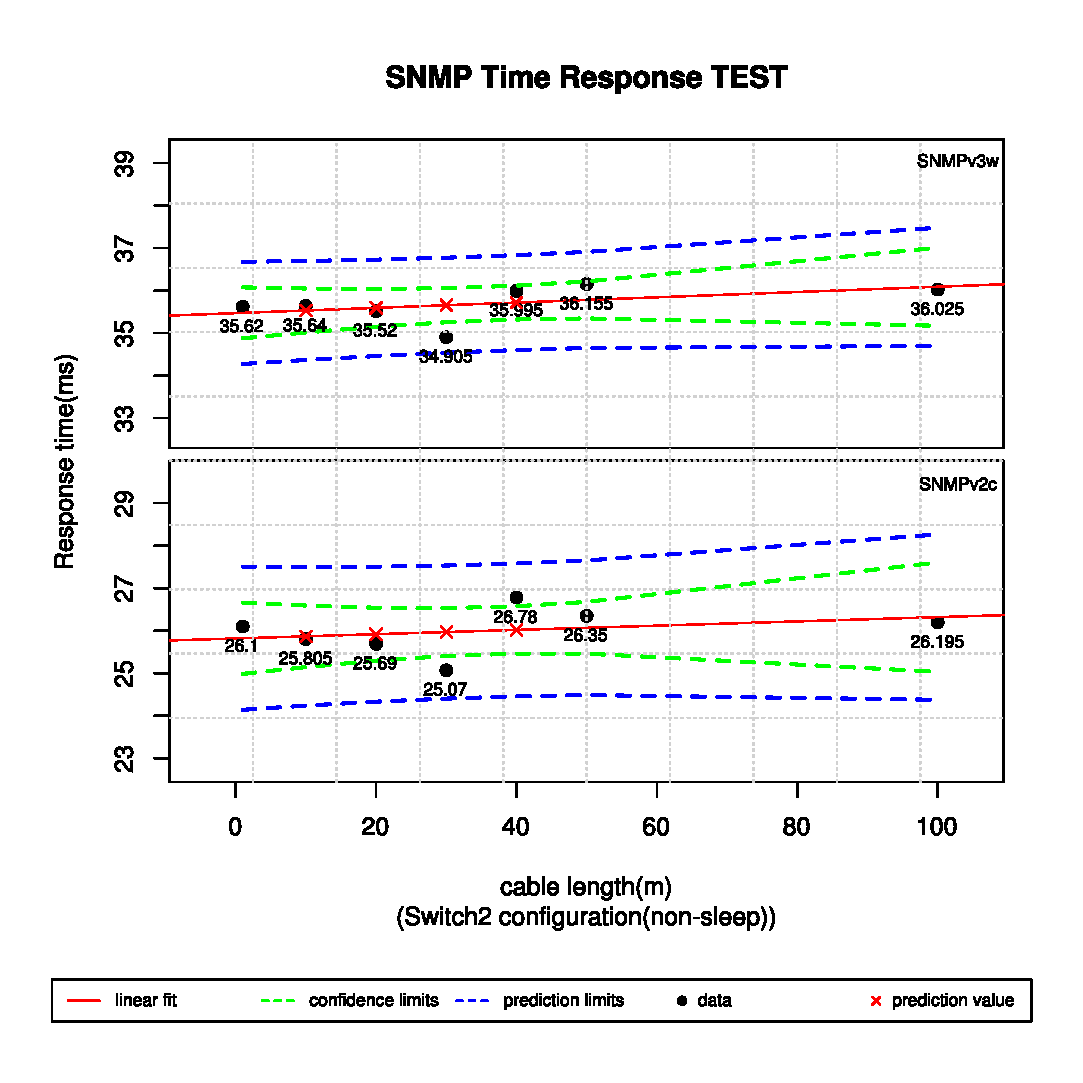
\includegraphics[width=0.5\textwidth]{./images/s2sx.eps}
  \caption{회귀분석 그래프 스위치 2개/Sleepx}
\end{figure}
 \begin{figure}[!htb]
  \centering
  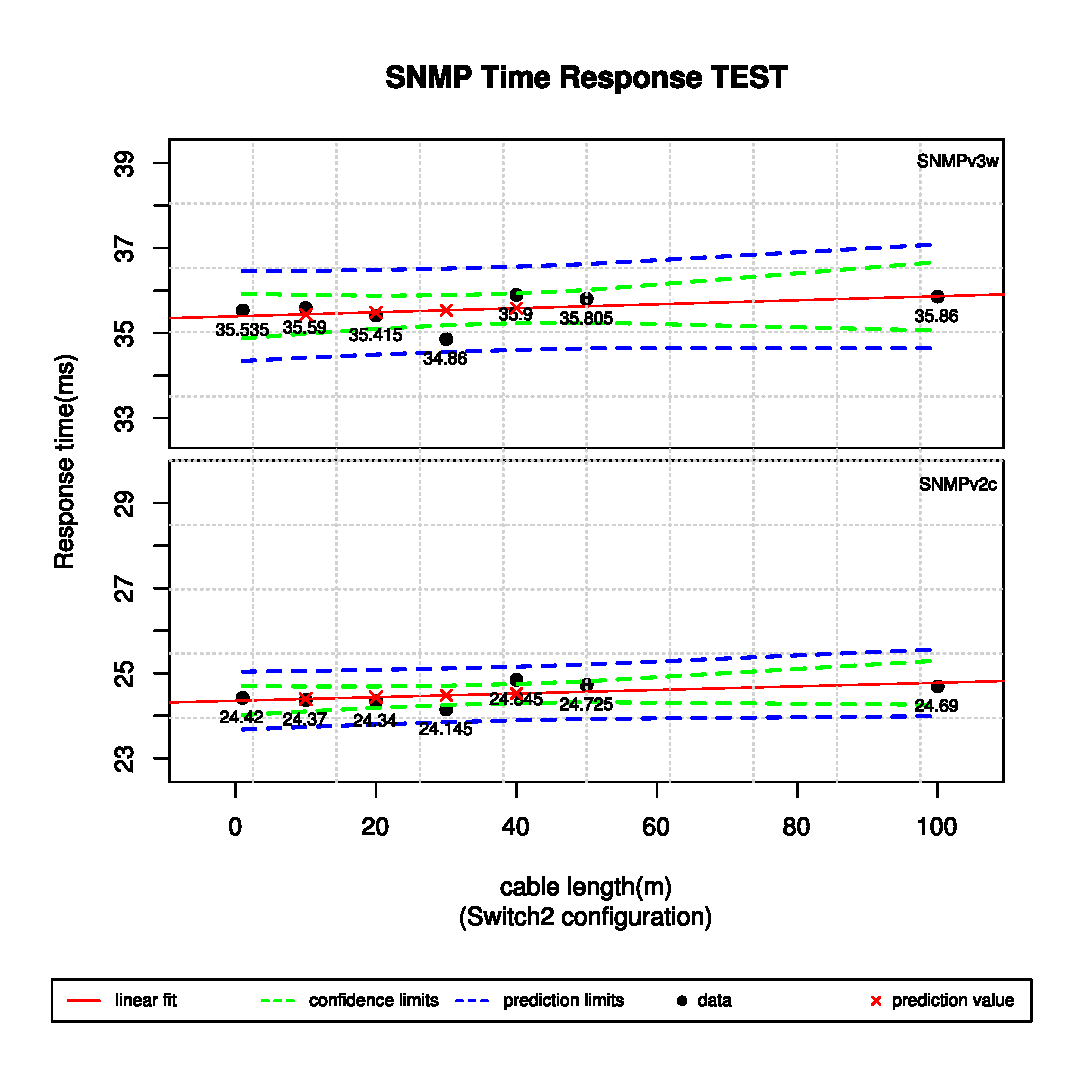
\includegraphics[width=0.5\textwidth]{./images/s2s1.eps}
  \caption{회귀분석 그래프 스위치 2개/Sleep1}
\end{figure}


\clearpage

\subsection{4.1.3 스위치 3개}
 \begin{figure}[!htb]
  \centering
  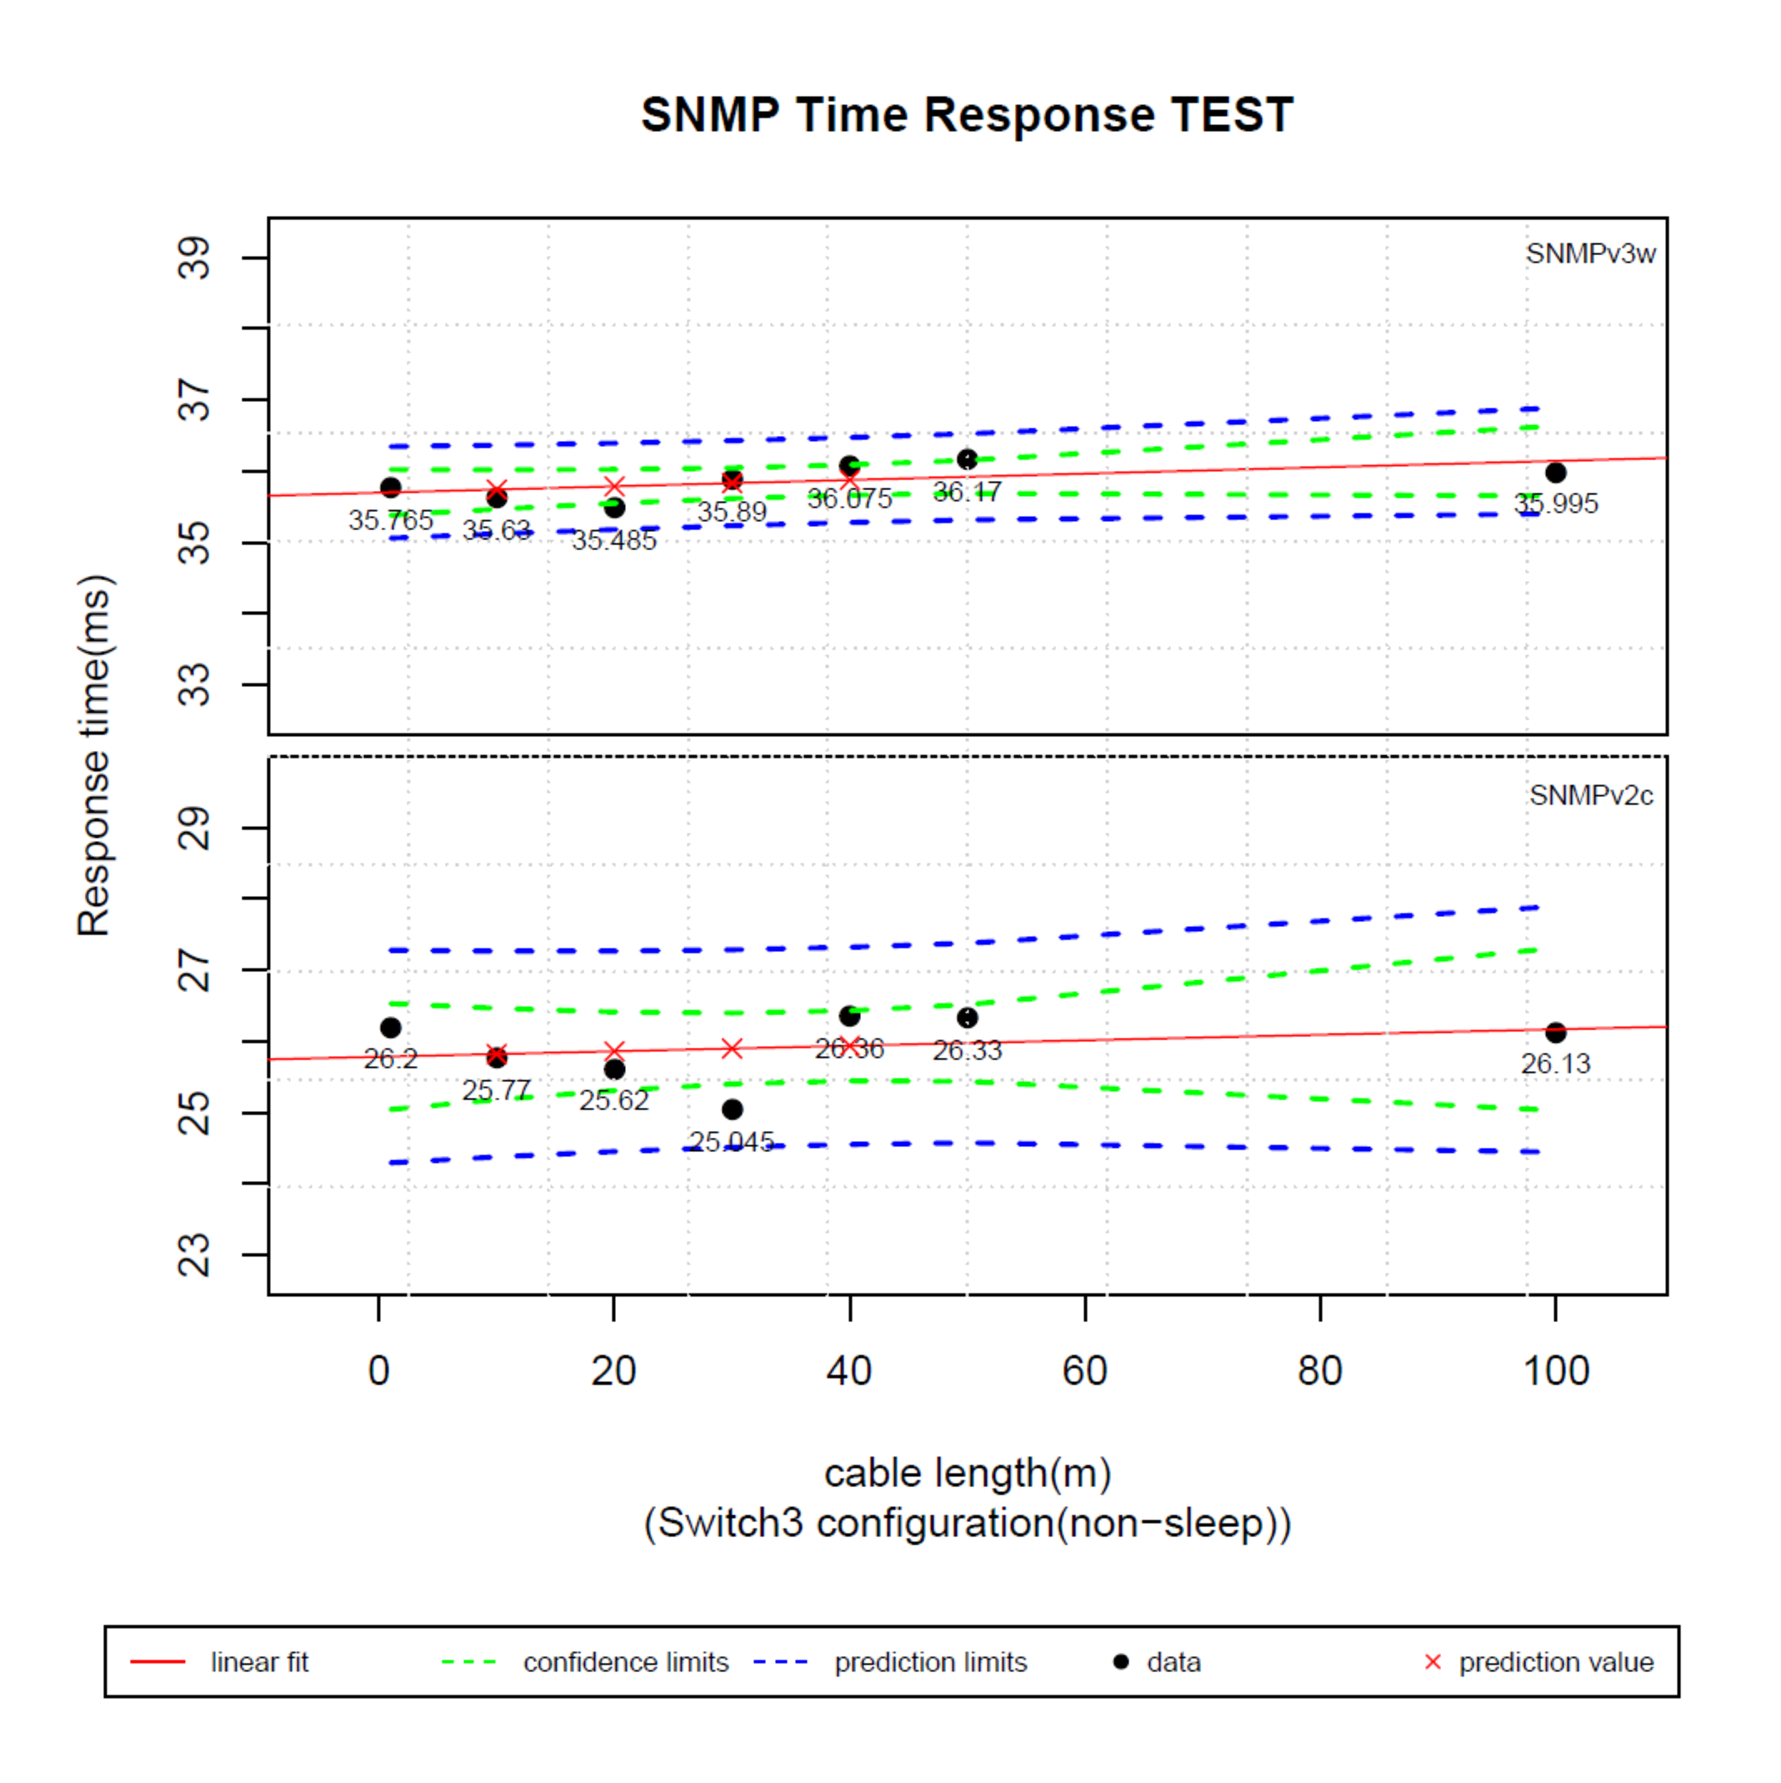
\includegraphics[width=0.5\textwidth]{./images/s3sx.eps}
  \caption{회귀분석 그래프 스위치 3개/Sleepx}
\end{figure}
 \begin{figure}[!htb]
  \centering
  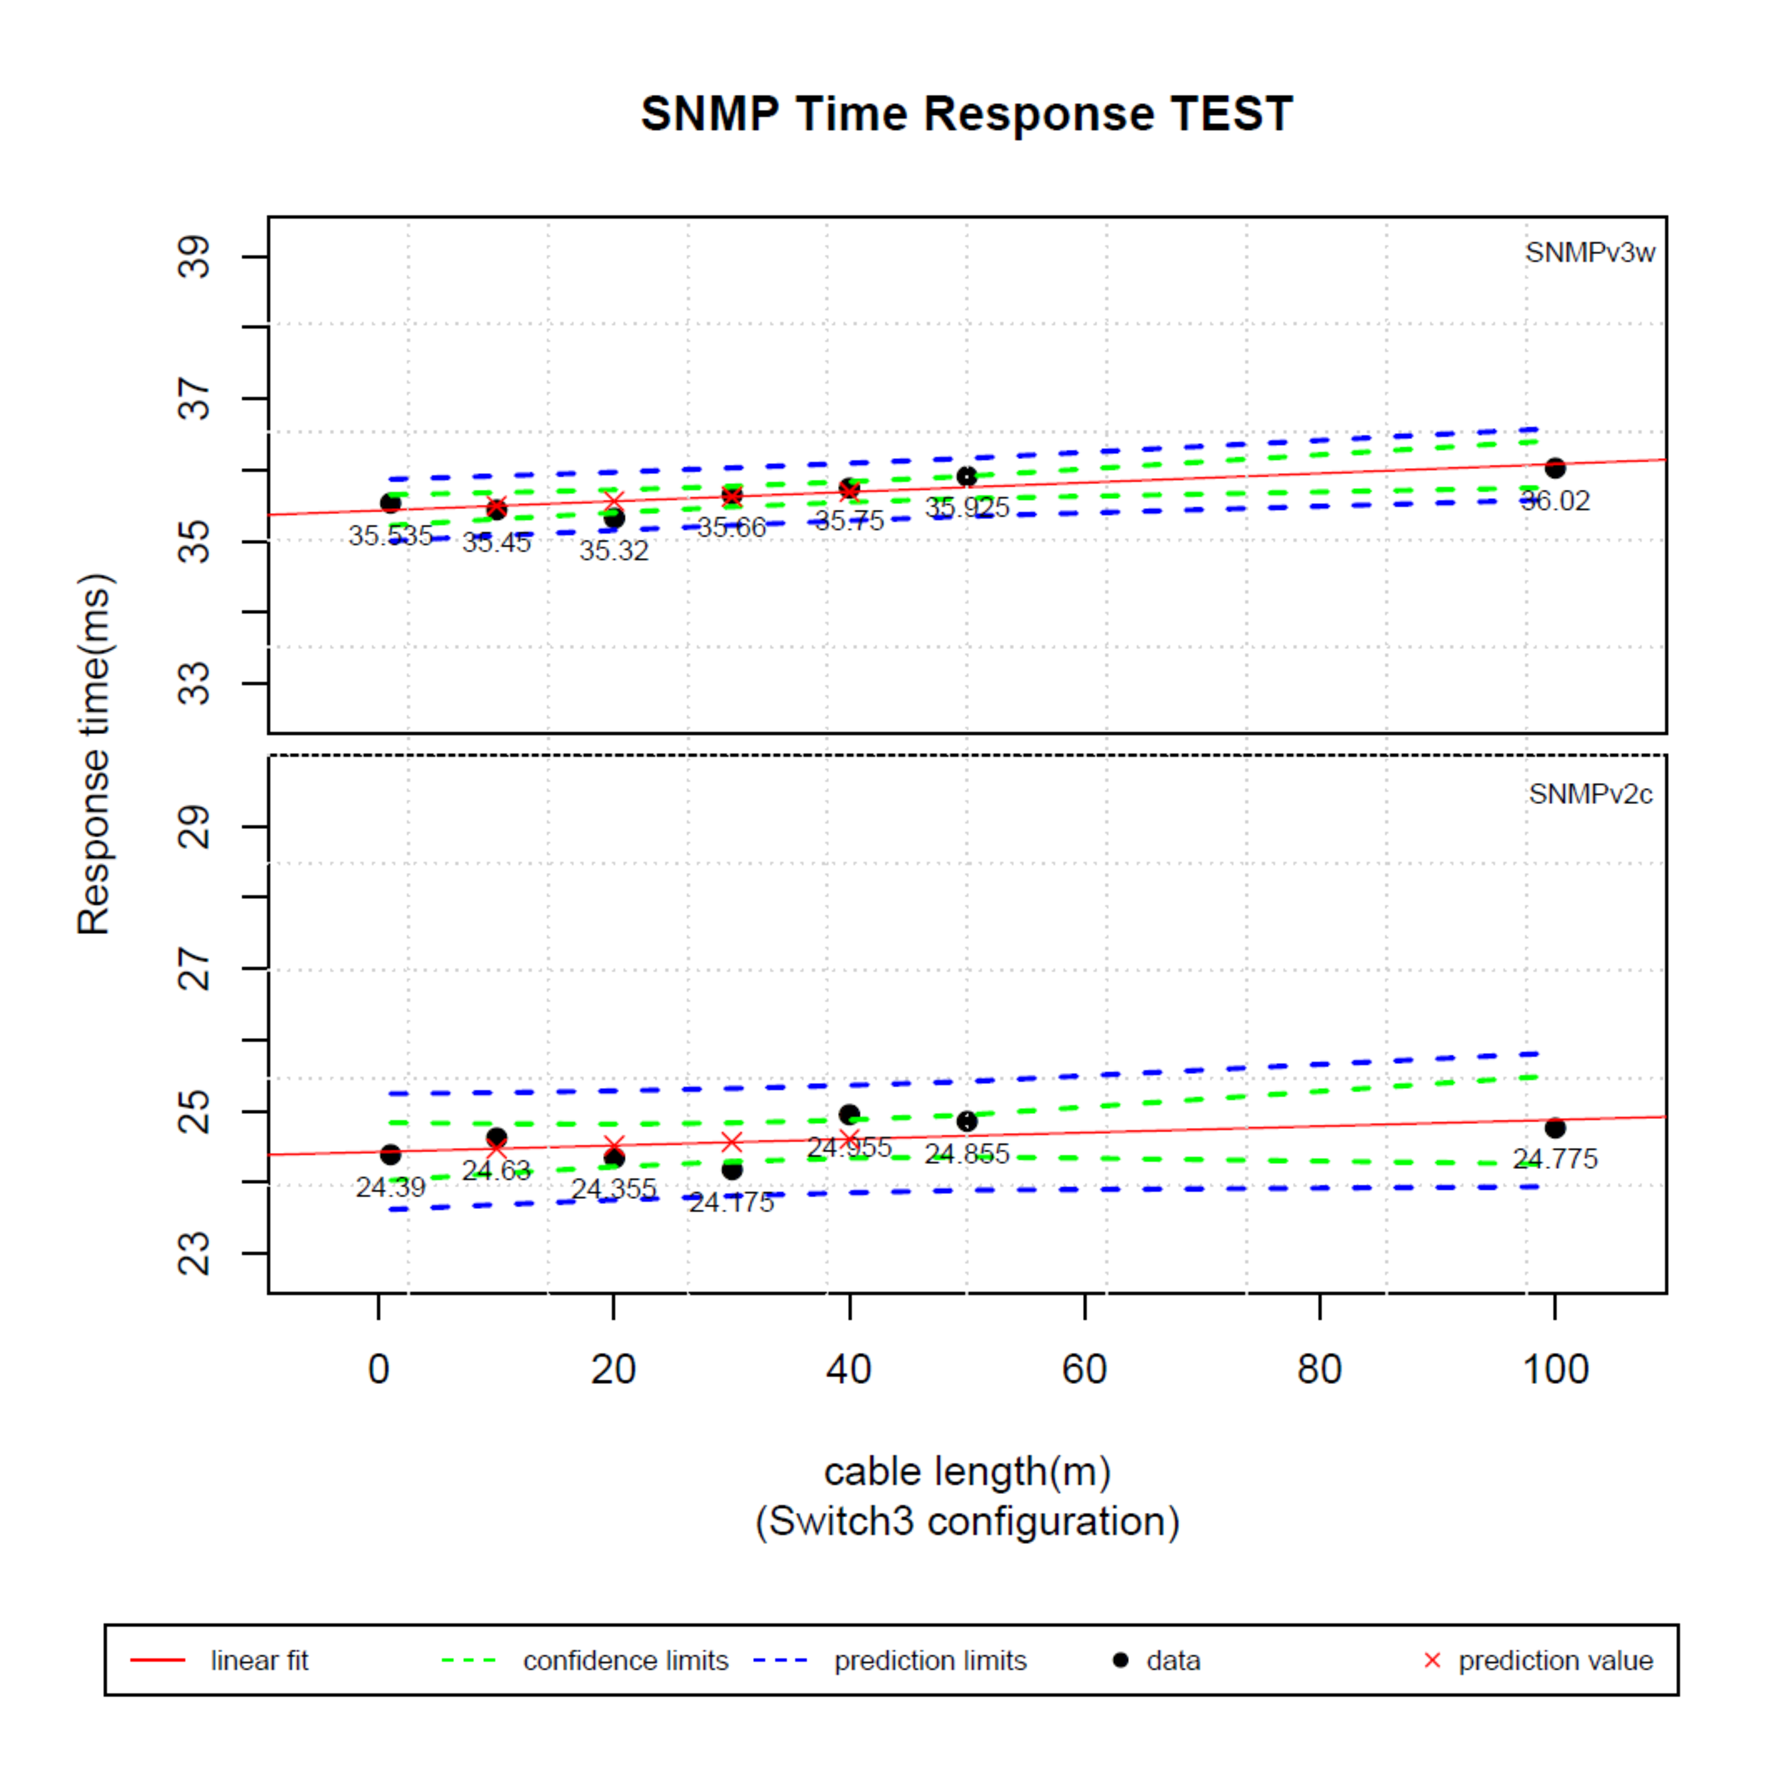
\includegraphics[width=0.5\textwidth]{./images/s3s1.eps}
  \caption{회귀분석 그래프 스위치 3개/Sleep1}
\end{figure}

\clearpage

\subsection{4.1.4 스위치 4개}
 \begin{figure}[!htb]
  \centering
  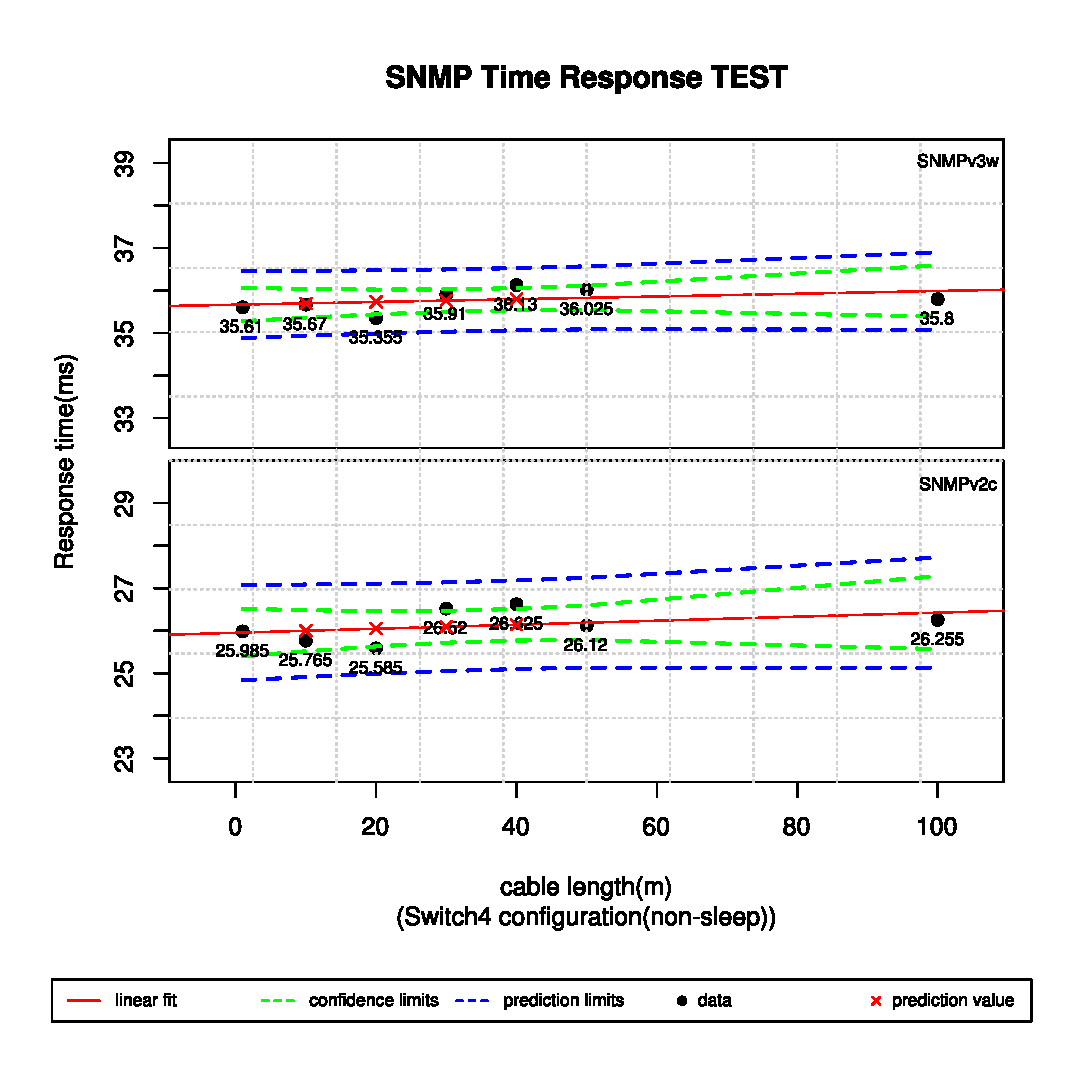
\includegraphics[width=0.5\textwidth]{./images/s4sx.eps}
  \caption{회귀분석 그래프 스위치 4개/Sleepx}
\end{figure}
 \begin{figure}[!htb]
  \centering
  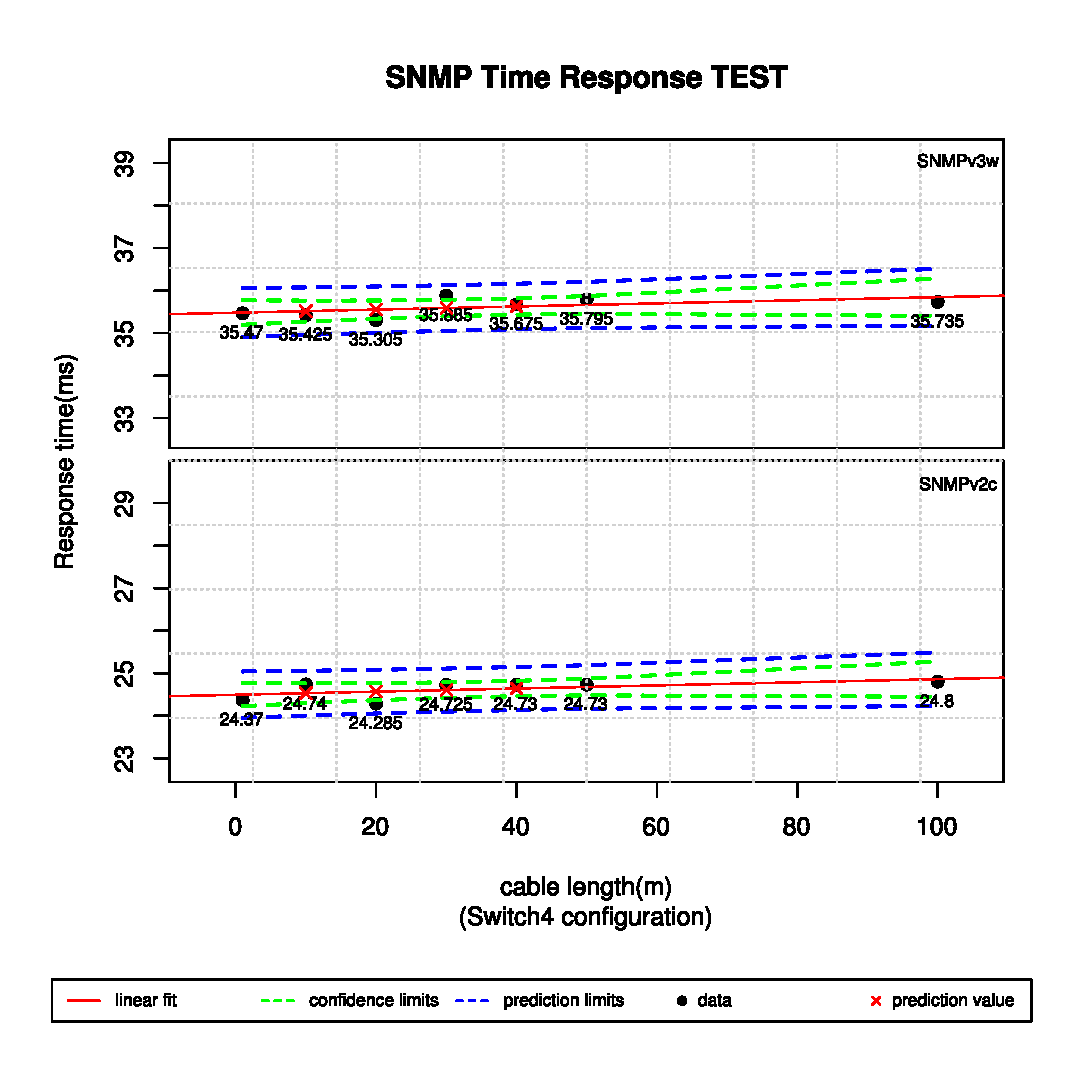
\includegraphics[width=0.5\textwidth]{./images/s4s1.eps}
  \caption{회귀분석 그래프 스위치 4개/Sleep1}
\end{figure}

\clearpage

\subsection{4.1.5 스위치 5개}
 \begin{figure}[!htb]
  \centering
  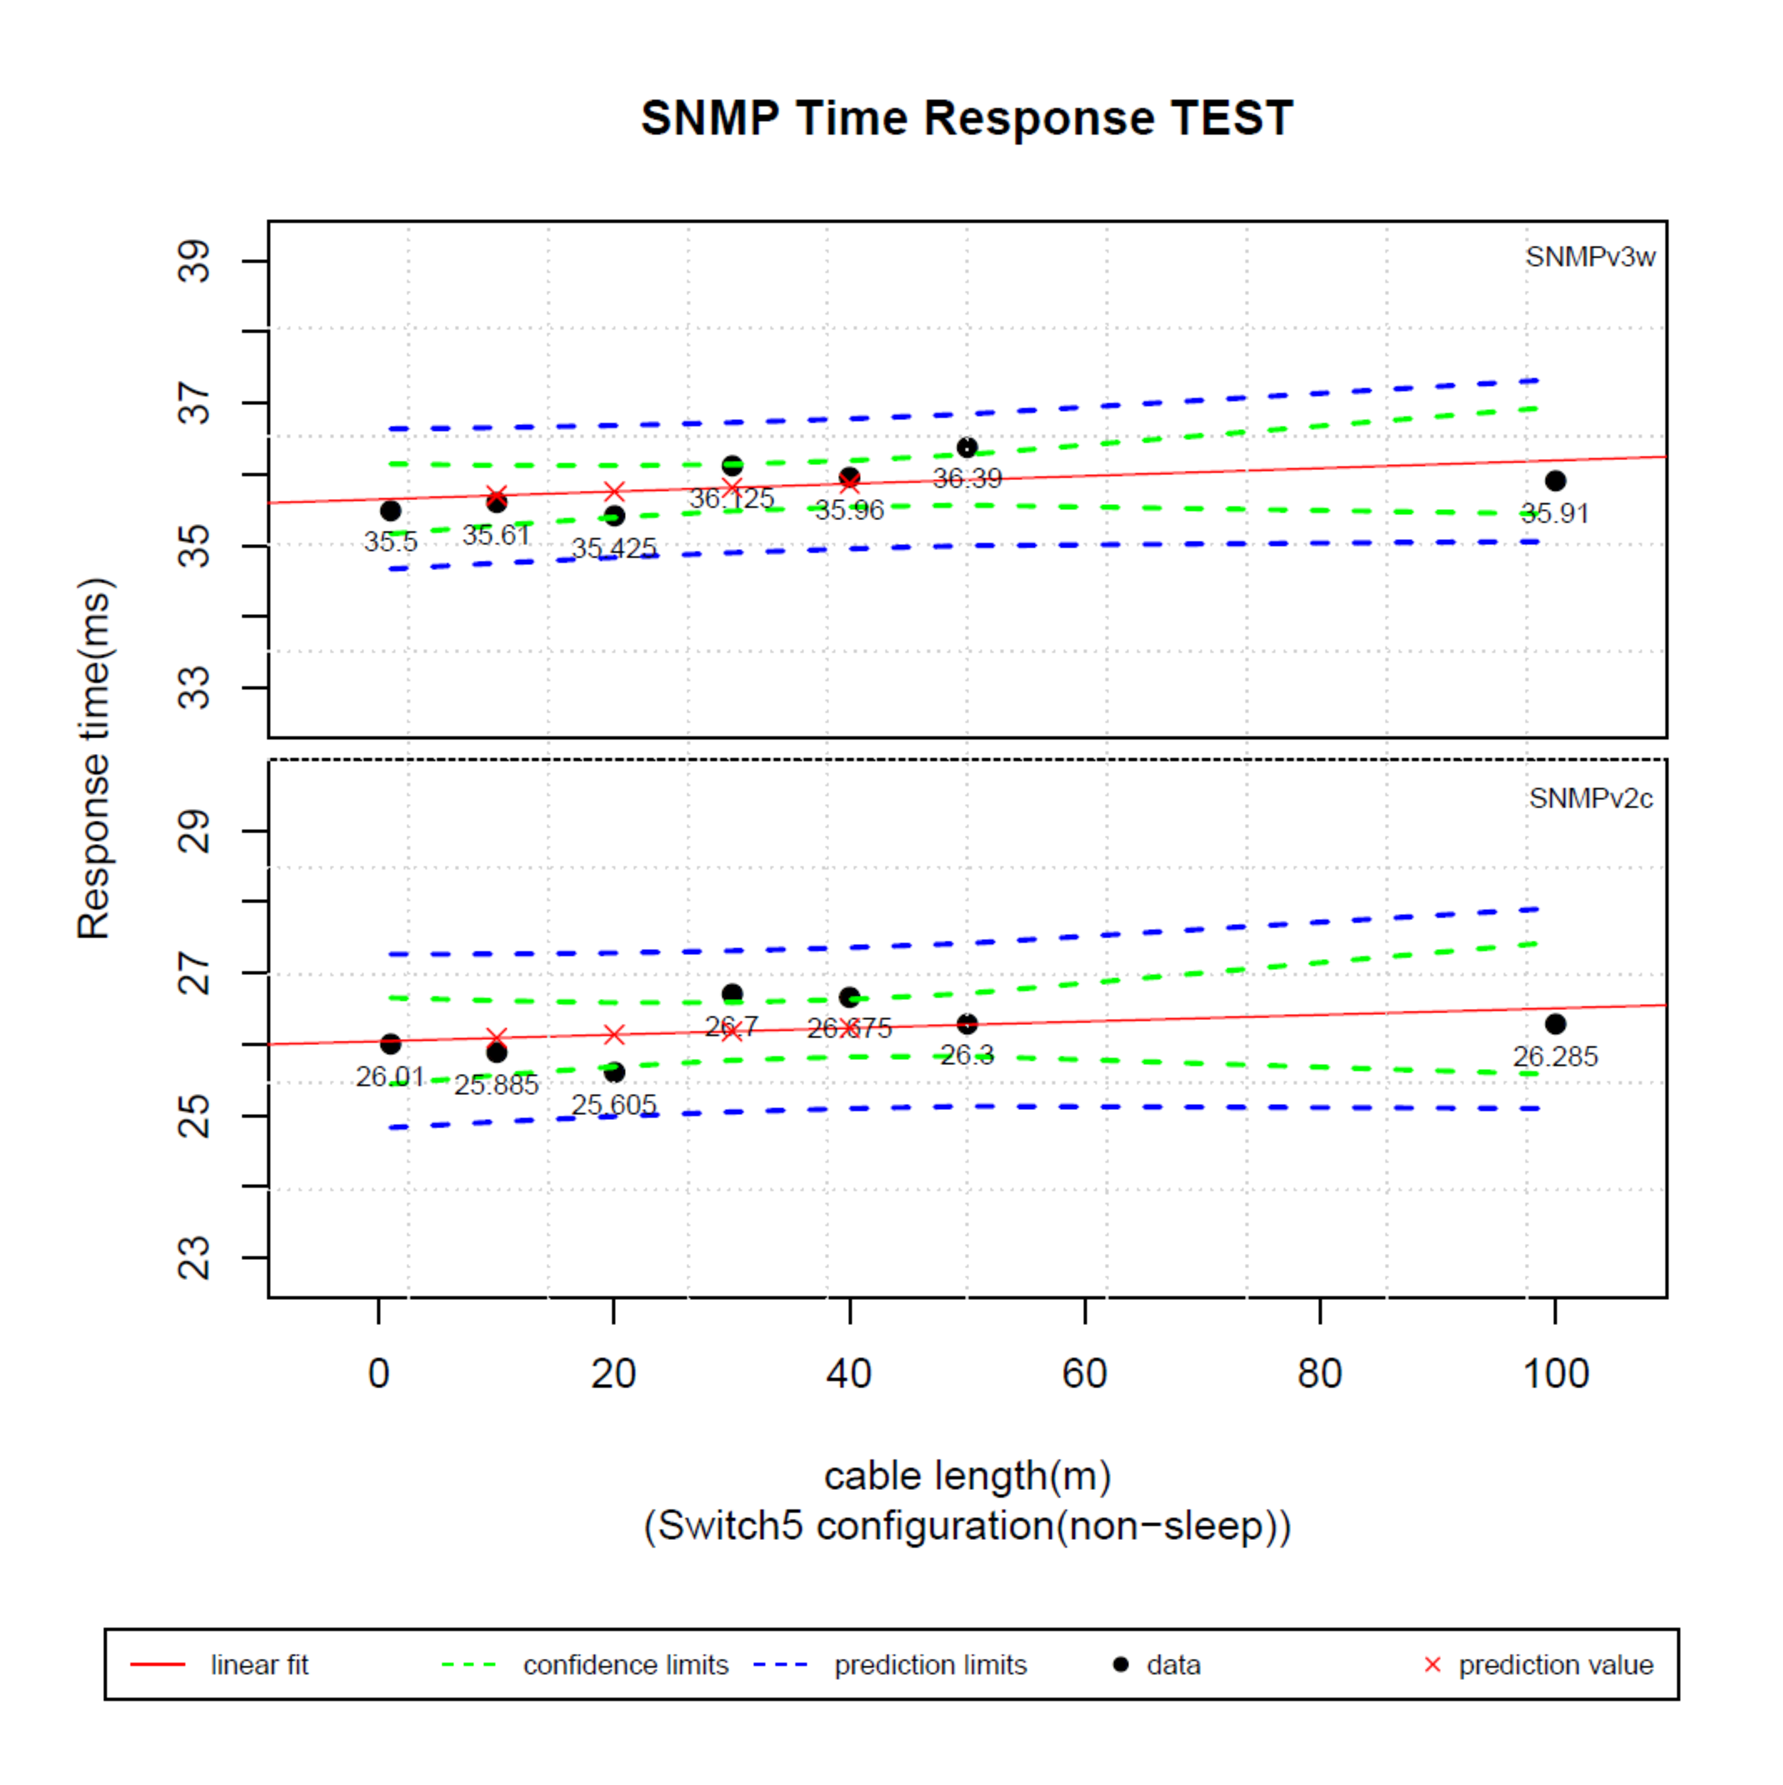
\includegraphics[width=0.5\textwidth]{./images/s5sx.eps}
  \caption{회귀분석 그래프 스위치 5개/Sleepx} 
\end{figure}
 \begin{figure}[!htb]
  \centering
  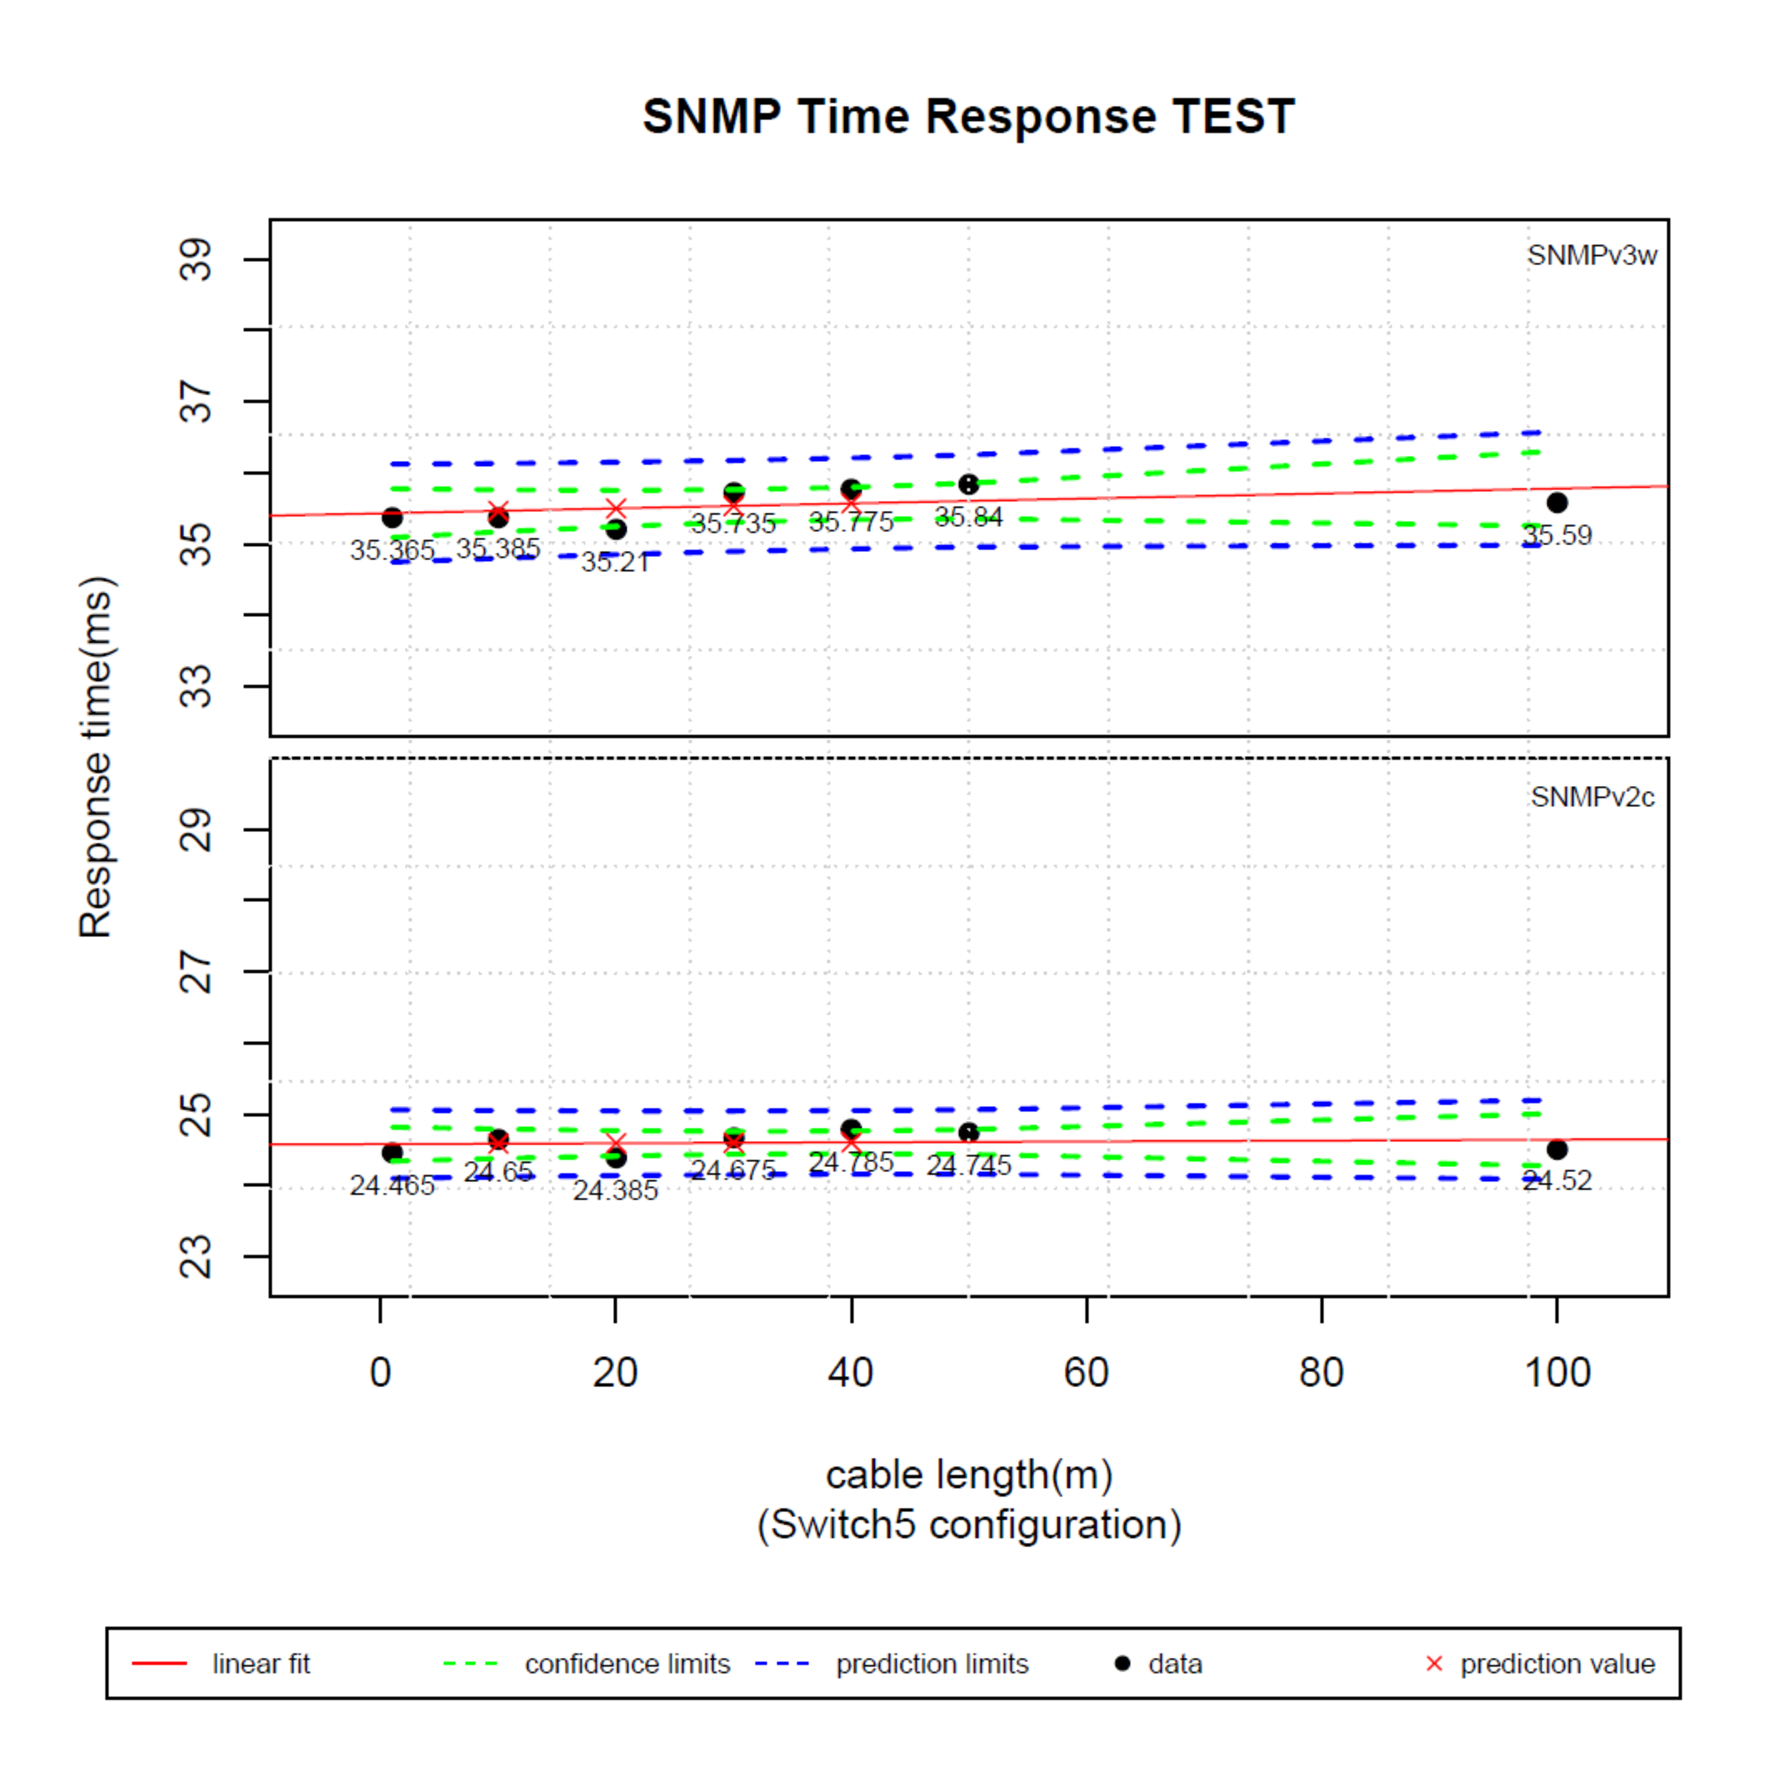
\includegraphics[width=0.5\textwidth]{./images/s5s1.eps}
  \caption{회귀분석 그래프 스위치 5개/Sleep1}
\end{figure}


\clearpage
\section{회귀분석 결과}\label{txt:result}  
\subsection{4.2.1 스위치 1개}

\begin{table}[h!]
\begin{center}
\begin{tabular}{c|c||c||c||c}\hline
\multicolumn{5}{c}{switch1/sleepx}\\ \hline\hline
\multicolumn{1}{c|}{}& \multicolumn{4}{c}{value}\\
\cline{1-5}
Independent variable & v1 & v2c & v3r & v3w      \\ \hline\hline
p-value &  0.164 &  0.166 & 0.105  &  0.111\\ 
F-value &  2.65 &  2.63&  3.9 &  3.73\\ 
R2 &  0.347  &  0.344&  0.438 &  0.427\\ 
Adjusted R2 & 0.0216 & 0.213 & 0.326 & 0.313\\ \hline\hline
\multicolumn{5}{r}{*p < 0.05} \\ \hline \hline
\multicolumn{5}{c}{switch1/sleep1}\\ \hline\hline
\multicolumn{1}{c|}{}& \multicolumn{4}{c}{value}\\
\cline{1-5}
Independent variable & v1 & v2c & v3r & v3w     \\ \hline\hline
p-value &  0.0802 &  0.0176& 0.464 &  0.231\\ 
F-value &  4.79  &  12.1&  0.628 &  1.86\\ 
R2 &  0.489 &  0.708 &  0.112  &  0.271\\ 
Adjusted R2 & 0.387 & 0.65 & -0.0661 & 0.125\\ \hline
\multicolumn{5}{r}{*p < 0.05} \\ \hline\hline
\end{tabular}
\caption{ 스위치 1개 회귀분석결과 }
\end{center}
\end{table} 

\clearpage
\subsection{4.2.2 스위치 2개}

\begin{table}[h!]
\begin{center}
\begin{tabular}{c|c||c||c||c}\hline
\multicolumn{5}{c}{switch2/sleepx}\\ \hline\hline
\multicolumn{1}{c|}{}& \multicolumn{4}{c}{value}\\
\cline{1-5}
Independent variable & v1 & v2c & v3r & v3w      \\ \hline\hline
p-value & 0.293 & 0.508 & 0.263 & 0.272\\ 
F-value & 1.38 & 0.507 & 1.59 & 1.52\\ 
R2 & 0.217 & 0.092 & 0.242 & 0.233\\ 
Adjusted R2 & 0.0598 & -0.0896 & 0.09 & 0.0799\\ \hline\hline
\multicolumn{5}{r}{*p < 0.05} \\ \hline \hline
\multicolumn{5}{c}{switch2/sleep1}\\ \hline\hline
\multicolumn{1}{c|}{}& \multicolumn{4}{c}{value}\\
\cline{1-5}
Independent variable & v1 & v2c & v3r & v3w      \\ \hline\hline
p-value &  0.294 &  0.179& 0.235  &  0.335\\ 
F-value &  1.38 &  2.22 &  1.82  &  1.14\\ 
R2 &  0.216 &  0.307&  0.267 & 0.185\\ 
Adjusted R2 & 0.059 & 0.169 & 0.121 & 0.0224\\ \hline
\multicolumn{5}{r}{*p < 0.05} \\ \hline\hline
\end{tabular}
\caption{  스위치 2개 회귀분석결과 }
\end{center}
\end{table} 

\clearpage
\subsection{4.2.3 스위치 3개}

\begin{table}[h!]
\begin{center}
\begin{tabular}{c|c||c||c||c}\hline
\multicolumn{5}{c}{switch3/sleepx}\\ \hline\hline
\multicolumn{1}{c|}{}& \multicolumn{4}{c}{value}\\
\cline{1-5}
Independent variable & v1 & v2c & v3r & v3w      \\ \hline\hline
p-value & 0.336 & 0.563 & 0.115 & 0.158\\ 
F-value & 1.13  & 0.383 & 3.62 & 2.75\\ 
R2 & 0.184 & 0.0711 & 0.42 & 0.355\\ 
Adjusted R2 & 0.0211 & -0.115 & 0.304 & 0.225\\ \hline\hline
\multicolumn{5}{r}{*p < 0.05} \\ \hline \hline
\multicolumn{5}{c}{switch3/sleep1}\\ \hline\hline
\multicolumn{1}{c|}{}& \multicolumn{4}{c}{value}\\
\cline{1-5}
Independent variable & v1 & v2c & v3r & v3w      \\ \hline\hline
p-value & 0.154 & 0.243 & 0.33 & 0.0155\\ 
F-value & 2.82 & 1.75 & 1.16 & 13\\ 
R2 & 0.361 & 0.259 & 0.189 & 0.722\\ 
Adjusted R2 & 0.233  & 0.111& 0.0262 & 0.666\\ \hline

\multicolumn{5}{r}{*p < 0.05} \\ \hline\hline
\end{tabular}
\caption{  스위치 3개 회귀분석결과 }
\end{center}
\end{table} 

\clearpage
\subsection{4.2.4 스위치 4개}

\begin{table}[h!]
\begin{center}
\begin{tabular}{c|c||c||c||c}\hline
\multicolumn{5}{c}{switch4/sleepx}\\ \hline\hline
\multicolumn{1}{c|}{}& \multicolumn{4}{c}{value}\\
\cline{1-5}
Independent variable & v1 & v2c & v3r & v3w      \\ \hline\hline
p-value &  0.409 & 0.36 & 0.419 & 0.374\\ 
F-value &  0.813 & 1.01 & 0.775 & 0.954\\ 
R2 & 0.14 & 0.169 & 0.134 & 0.16\\ 
Adjusted R2 & -0.0322 & 0.00245 & -0.039 & -0.00774\\ \hline\hline
\multicolumn{5}{r}{*p < 0.05} \\ \hline \hline
\multicolumn{5}{c}{switch4/sleep1}\\ \hline\hline
\multicolumn{1}{c|}{}& \multicolumn{4}{c}{value}\\
\cline{1-5}
Independent variable & v1 & v2c & v3r & v3w      \\ \hline\hline
p-value & 0.000107 & 0.168 & 0.112 & 0.19\\ 
F-value & 122 &  2.59&  3.7  &  2.3\\ 
R2 & 0.961 & 0.342& 0.426 & 0.315\\ 
Adjusted R2 & 0.953 & 0.21& 0.311 & 0.178\\ \hline

\multicolumn{5}{r}{*p < 0.05} \\ \hline\hline
\end{tabular}
\caption{  스위치 4개 회귀분석결과 }
\end{center}
\end{table} 

\clearpage
\subsection{4.2.5 스위치 5개}

\begin{table}[h!]
\begin{center}
\begin{tabular}{c|c||c||c||c}\hline
\multicolumn{5}{c}{switch5/sleepx}\\ \hline\hline
\multicolumn{1}{c|}{}& \multicolumn{4}{c}{value}\\
\cline{1-5}
Independent variable & v1 & v2c & v3r & v3w      \\ \hline\hline
p-value & 0.616 & 0.405& 0.159 & 0.242\\ 
F-value & 0.285 & 0.828& 2.74 & 1.76\\ 
R2 & 0.054 & 0.142& 0.354 & 0.26\\ 
Adjusted R2 & -0.135 & -0.0295& 0.224 & 0.112\\ \hline\hline
\multicolumn{5}{r}{*p < 0.05} \\ \hline \hline
\multicolumn{5}{c}{switch5/sleep1}\\ \hline\hline
\multicolumn{1}{c|}{}& \multicolumn{4}{c}{value}\\
\cline{1-5}
Independent variable & v1 & v2c & v3r & v3w      \\ \hline\hline
p-value & 0.751 & 0.768 & 0.595 & 0.28\\ 
F-value & 0.113 & 0.0968 & 0.323 & 1.47\\ 
R2 & 0.022 & 0.01 9& 0.0606 & 0.227\\ 
Adjusted R2 & -0.174 & -0.177 & -0.127 & 0.072\\ \hline

\multicolumn{5}{r}{*p < 0.05} \\ \hline\hline
\end{tabular}
\caption{  스위치 5개 회귀분석결과 }
\end{center}
\end{table} 





\clearpage
\bibliographystyle{unsrtnat}
\bibliography{./refs}


\end{document}

